\chapter{SISTEMA WEB KEEME} 
\label{chap:proposta}

O KeeMe (Keep it to Me, "Guarde isso para mim") nasceu de uma necessidade da Faculdade de Computação e Engenharia Elétrica de informatizar o processo de validação das ACCs realizadas pelos discentes. Dessa forma, o sistema fará o armazenamento dos certificados gerados pelos discentes, e calculará os pontos gerados por essas ACCs. O objetivo principal da ferramenta é simplificar o processo de validação dos certificados por parte da faculdade, diminuindo a burocracia necessária para a avaliação, e dar aos discentes um acompanhamento de quantos pontos eles já obtiveram e em quais modalidades de ACCs eles podem adquirir mais pontos.

A Seção \ref{sec:coleta_de_requisitos} descreverá a etapa de coleta e análise de requisitos do sistema, feita com as partes interessadas do sistema. Já a Seção \ref{sec:modelagemDeRequisitos} irá discorrer sobre a etapa de modelagem dos requisitos coletados em representações gráficas. A arquitetura do sistema será mostrada na Seção \ref{sec:arquiteturaDoSistema} que explicará a forma em que o sistema foi estruturado. E por último a Seção \ref{sec:implementacao} explanará sobre a implementação da ferramenta, mostrando as funcionalidades que foram criadas.

\section{Coleta de Requisitos}
\label{sec:coleta_de_requisitos}

O autor de \cite{pmbok2017} descreve a etapa de coleta e análise de requisitos como "o processo de determinar, documentar e gerenciar as necessidades e requisitos das partes interessadas a fim de cumprir os objetivos". Dessa forma, requisitos de um software são todas as necessidades que as partes interessadas possuem dentro de um determinado escopo e que devem ser resolvidas através do desenvolvimento de uma aplicação. Através de reuniões e da análise do documento referente à pontuação de carga horária de ACCs que pode ser encontrado no Anexo \ref{anexo:novaResolucaoDeACC}, foram elencados requisitos funcionais e não funcionais, listados de acordo com o grau de prioridade.

Os requisitos levantados foram divididos entre requisitos funcionais, que de acordo com \cite{pmbok2017} descrevem os comportamentos do produto, ou seja, são as ações diretas que os usuários do sistema realizarão e a forma que o sistema reagira a elas; e não funcionais, são todos aqueles em que não há interação direta por parte do usuário, e que estão relacionados à infraestrutura por trás da aplicação, descritos como uma complementação dos requisitos funcionais que descrevem as condições ou qualidades ambientais requeridas para que o produto seja eficaz.

A Tabela \ref{table:RequisitosFuncionais} lista a relação dos requisitos funcionais coletados. Os requisitos estão classificados por ordem de prioridade como "essencial" sendo algo que deve obrigatoriamente ser desenvolvido no sistema, "importante" como algo que agregaria mais valor ao sistema, mas que não interfere na utilização e "desejável" como sendo algo além daquilo que a aplicação já se propõe a fazer, e que não interfere de forma alguma em seu funcionamento.

\begin{table}[H]
\centering
\caption{Requisitos Funcionais}
\label{table:RequisitosFuncionais}
\begin{tabular}{|C{1.2cm}|C{11.2cm}|C{2.2cm}|}
\hline
\textbf{ID} & \textbf{Descrição} & \textbf{Prioridade} \\
\hline
RF 1 & O usuário poderá fazer login no sistema. & Essencial \\ \hline
RF 2 & O discente poderá gerenciar as pontuações dos respectivos ACCs. & Essencial \\ \hline
RF 3 & O discente poderá enviar os certificados digitalmente pela plataforma. & Essencial \\ \hline
RF 4 & O sistema mostrará aos discentes o seu progresso na obtenção das ACCs. & Essencial \\ \hline
RF 5 & A pontuação do discente deverá obedecer os limites de cada tipo de ACC. & Essencial \\ \hline
RF 6 & A coordenação do curso poderá acompanhar as ACCs de cada discente. & Essencial \\ \hline
RF 7 & A coordenação do curso poderá validar os documentos enviados pelos discentes. & Essencial \\ \hline
RF 8 & A administração poderá gerenciar os dados referentes a ACC (pontuação, carga máxima, etc). & Importante \\ \hline
RF 9 & A coordenação poderá cadastrar o motivo caso um certificado de ACC seja negado. & Desejável \\ \hline
RF 10 & A coordenação poderá acompanhar o desempenho geral por turma na obtenção de ACC & Desejável \\ \hline
RF 11 & A coordenação poderá fazer a geração de relatórios das pontuações dos alunos & Desejável \\ \hline

\end{tabular}
\end{table}


Os requisitos não funcionais coletados e relacionados na Tabela \ref{table:RequisitosNaoFuncionais}, assim como os funcionais, estão classificados por ordem de prioridade como "essencial" sendo algo que deve obrigatoriamente ser desenvolvido no sistema e que é essencial para o seu funcionamento, "importante" como algo que agregaria mais valor ao sistema, mas que não interfere diretamente no seu funcionamento final, e "desejável" como sendo algo que poderia ser implementador na arquitetura da aplicação, porém não interfere de forma alguma em seu funcionamento final.

\begin{table}[H]
\centering
\caption{Requisitos Não Funcionais}
\label{table:RequisitosNaoFuncionais}
\begin{tabular}{|C{1.2cm}|C{11.2cm}|C{2.2cm}|}
\hline
\textbf{ID} & \textbf{Descrição} & \textbf{Prioridade} \\
\hline
RNF 1 & O sistema deverá possuir autenticação e uso de \textit{tokens} de forma a garantir a segurança dos usuários. & Essencial \\ \hline
RNF 2 & O deverá possuir criptografia das senhas dos usuários. & Essencial \\ \hline
RNF 3 & O sistema deverá estar disponível a todo momento. & Essencial \\ \hline
RNF 4 & O sistema deverá ser responsivo, com foco na utilização em dispositivos móveis. & Essencial \\ \hline
RNF 5 & O sistema deverá ter suporte para os principais navegadores, sendo estes: Chrome, Firefox, Safari, Microsoft Edge. & Importante \\ \hline
RNF 6 & Deverão ser seguidas as principais heurísticas de Interface Homem Computador de forma a garantir a usabilidade do sistema. & Importante \\ \hline
RNF 7 & Deverá haver o suporte a um PWA do sistema & Desejável \\ \hline
RNF 8 & Deverá possuir código HTML escrito de forma semântica de forma a permitir acessibilidade. & Desejável \\ \hline

\end{tabular}
\end{table}

\section{Modelagem de Requisitos}
\label{sec:modelagemDeRequisitos}

O objetivo da etapa de modelagem de requisitos é transformar os requisitos coletados pelas partes interessadas em artefatos que sejam compreensíveis visualmente à equipe de desenvolvimento. \cite{pressman2009engenharia} descreve a modelagem como sendo algo que ”abrange tanto análise quanto projeto, descrevendo representações do \textit{software} que se tornam progressivamente mais detalhadas”. Essas representações são essenciais para que se saiba exatamente o que se deve ser desenvolvido dentro de um \textit{software}.

\subsection{Casos de Uso de Alto Nível e Expandido}

O autor \cite{guedes2018uml} descreve os casos de uso como diagramas que procuram por meio de uma linguagem simples demonstrar as funcionalidades de um sistema para os usuários, possibilitando uma melhor compreensão por parte daqueles que não entendem completamente o funcionamento interno do sistema. Diagramas de caso de uso servem então para mostrar quais são os atores de um sistema, sendo esses atores os tipos de usuários, e quais as ações que cada um desses atores podem realizar. Dentro do contexto do KeeMe, existem os seguintes atores:
\begin{itemize}
    \item Discente: é o ator que representa um discente no sistema, ele possui a capacidade de fazer a gestão das ACCs assim como de visualizar a pontuação que já obteve.
    \item Coordenador: usuário capaz de realizar as avaliações de ACC dentro do sistema, assim como de visualizar as pontuações dos alunos.
    \item Administrador: é o usuário que faz o gerenciamento dos tipos de ACC presentes no sistema, assim como dos coordenadores;
\end{itemize}

\begin{figure}[H]
    \centering
    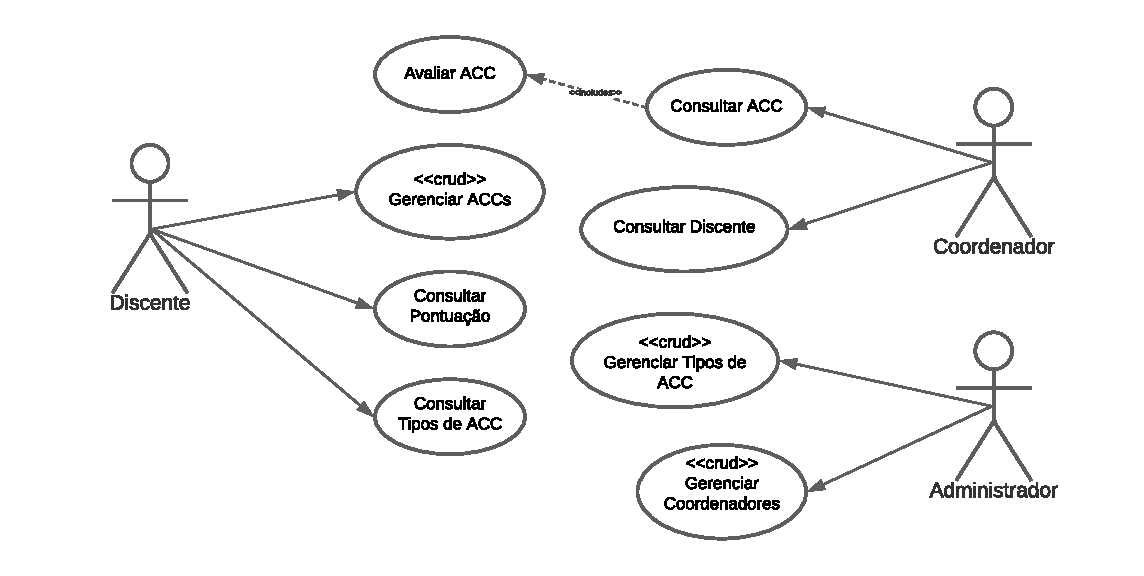
\includegraphics[width=\textwidth]{dados/figuras/Proposta/casos_de_uso_de_alto_nivel__keeme.pdf}
    \caption{Diagrama de Caso de Uso de Alto Nível do KeeMe.}
    \label{fig:casoDeUsoAltoNivel}
\end{figure}

Os casos de uso também podem ser expandidos textualmente em uma sequência de passos presentes dentro dos mesmos. A Tabela \ref{casoExpandido:consultarPontuacao} descreve o caso de uso onde o discente faz a consulta de sua pontuação no sistema, essa pontuação é referente à pontuação necessária para integralização da matéria de ACC; Já a Tabela \ref{casoExpandido:consultarTiposDeACC} demonstra a sequência de ações presentes no caso de uso de consulta dos tipos de ACC, onde o discente poderá acessar os tipos de ACC presentes no sistema; A Tabela \ref{casoExpandido:gerenciarACCs} também é referente às ações do discente, e diz respeito às ações de cadastro, consulta, edição e exclusão das ACCs de um discente.

Os casos de uso de um usuário do tipo coordenador estão listados nas Tabelas \ref{casoExpandido:consultarACC}, \ref{casoExpandido:avaliarACCs} e \ref{casoExpandido:consultarDiscentes}. A Tabela \ref{casoExpandido:consultarACC} descreve a consulta de uma ACC, onde o coordenador poderá acessar os detalhes de uma ACC enviada por um discente; Já a Tabela \ref{casoExpandido:avaliarACCs} descreve a sequência de passos para a avaliação de uma ACC, como mostrado na Figura \ref{fig:casoDeUsoAltoNivel} essa ação inclui o caso de uso de Consultar ACC, descrito na tabela \ref{casoExpandido:consultarACC}; Além disso, a Tabela \ref{casoExpandido:consultarDiscentes} descreve a consulta de discentes que pode ser feita por um coordenador, esta busca retorna os discentes que contenham o campo usado na pesquisa e que sejam do mesmo curso do coordenador, através desse caso de uso os coordenadores podem acessar os detalhes dos dados e pontuação dos discentes.

Enquanto isso os casos de uso de um administrador estão presentes nas Tabelas \ref{casoExpandido:gerenciarTiposDeACC}, que descreve o gerenciamento dos Tipos de ACC, descrevendo o fluxo de cadastro, consulta, edição e exclusão dos mesmos; e \ref{casoExpandido:gerenciarCoordenadores}, que descreve as ações de cadastro, consulta, edição e exclusão dos coordenadores do sistema, ação que só pode ser realizada por um administrador.

%  CASOS EXPANDIDOS : DISCENTE ------------------------------

\begin{table}[H]
\caption{Caso de Uso Expandido - Consultar Pontuação}
\label{casoExpandido:consultarPontuacao}
\begin{tabular}{p{0.25\textwidth}p{0.693\textwidth}}
\hline
\textbf{Item}               & \textbf{Descrição} \\
\hline
\textbf{Caso de Uso:}       & Consultar Pontuação \\
\textbf{Ator:}              & Discente \\

\textbf{Fluxo Principal:}   & \begin{tabular}{@{}p{0.68\textwidth}}1. O discente seleciona a opção de consultar pontuação\\ 2. O sistema retorna a quantidade de pontos aprovados, reprovados e em análise do discente.\end{tabular} \\
\hline
\end{tabular}
\end{table}

\begin{table}[H]
\caption{Caso de Uso Expandido - Consultar Tipos de ACC}
\label{casoExpandido:consultarTiposDeACC}
\begin{tabular}{p{0.25\textwidth}p{0.693\textwidth}}
\hline
\textbf{Item}               & \textbf{Descrição} \\
\hline
\textbf{Caso de Uso:}       & Consultar Tipos de ACC \\
\textbf{Ator:}              & Discente \\

\textbf{Fluxo Principal:}   & \begin{tabular}{@{}p{0.68\textwidth}}1. O discente seleciona a opção de consultar tipos de ACC\\ 2. O sistema retorna ao discente os tipos de ACC presentes no sistema.\end{tabular} \\
\hline
\end{tabular}
\end{table}

\begin{table}[H]
\centering
\caption{Caso de Uso Expandido - Gerenciar ACCs}
\label{casoExpandido:gerenciarACCs}
\begin{tabular}{p{0.25\textwidth}p{0.693\textwidth}}
\hline
\textbf{Item}               & \textbf{Descrição} \\
\hline
\textbf{Caso de Uso:}       & Gerenciar ACCs  <{}<crud>{}>\\
\textbf{Ator:}              & Discente \\
\textbf{Fluxo Principal:}   & \begin{tabular}{@{}p{0.68\textwidth}}1. O discente seleciona a opção de Gerenciar ACCs.\\
2. O sistema mostra ao discente todas as ACCs cadastradas por ele.
3. O usuário escolhe entre uma das opções:
\begin{itemize}
    \item Inserir ACC: Variante 2a.
    \item Consultar ACC: Variante 2b.
    \item Atualizar ACC: Variante 2c.
    \item Excluir ACC: Variante 2d.
\end{itemize}
\end{tabular} \\

\multicolumn{2}{l}{\textbf{Variante 2a: Inserir ACC}} \\ \hline
& \begin{tabular}{@{}p{0.68\textwidth}}1. O discente preenche os campos de Tipo de ACC, Carga Horária, Descrição e Anexa um certificado.\\ 2. O discente submete o cadastro. \\ 4. O sistema encaminha a pontuação para ser avaliada por um Coordenador. \\ 5. O sistema retorna uma mensagem contendo o resultado do cadastro.
\end{tabular} \\

\multicolumn{2}{l}{\textbf{Variante 2b: Consultar ACC}} \\ \hline
& \begin{tabular}{@{}p{0.68\textwidth}} 1. O discente escolhe uma das ACCs \\ 2. O sistema retorna os detalhes da ACC.\\
\end{tabular} \\

\multicolumn{2}{l}{\textbf{Variante 2c: Atualizar ACC}} \\ \hline
& \begin{tabular}{@{}p{0.68\textwidth}}
1. O discente escolhe uma das ACCs. \\ 2. O sistema retorna os detalhes da ACC. \\ 3. O discente seleciona a opção de Editar ACC.\\ 4. O discente faz as alterações na pontuação. \\ 5. O discente submete as atualizações. \\ 6. O sistema retorna uma mensagem contendo o resultado da edição.
\end{tabular} \\

\multicolumn{2}{l}{\textbf{Variante 2d: Excluir ACC}} \\ \hline
& \begin{tabular}{@{}p{0.68\textwidth}}1. O discente escolhe uma das ACCs. \\ 2. O sistema os detalhes da ACC. \\ 3. O discente seleciona a opção de Excluir ACC.\\ 4. O sistema retorna uma mensagem do resultado da exclusão.
\end{tabular} \\
\end{tabular}
\end{table}

%  CASOS EXPANDIDOS : COORDENADOR ------------------------------

% Consultar ACC

\begin{table}[H]
\caption{Caso de Uso Expandido - Consultar ACC}
\label{casoExpandido:consultarACC}
\begin{tabular}{p{0.25\textwidth}p{0.693\textwidth}}
\hline
\textbf{Item}               & \textbf{Descrição} \\
\hline
\textbf{Caso de Uso:}       &  Consultar ACC \\
\textbf{Ator:}              & Coordenador \\

\textbf{Fluxo Principal:}   & \begin{tabular}{@{}p{0.68\textwidth}}1. O coordenador escolhe a opção de Consultar ACCs Recebidas\\ 2. O sistema mostra as requisições recebidas não avaliadas.\\ 3. O coordenador seleciona uma das ACCs. \\ 4. O sistema retorna os detalhes da ACC. \\ \end{tabular} \\
\hline
\end{tabular}
\end{table}

% Avaliar ACC

\begin{table}[H]
\caption{Caso de Uso Expandido - Avaliar ACC}
\label{casoExpandido:avaliarACCs}
\begin{tabular}{p{0.25\textwidth}p{0.693\textwidth}}
\hline
\textbf{Item}               & \textbf{Descrição} \\
\hline
\textbf{Caso de Uso:}       &  Avaliar ACC \\
\textbf{Ator:}              & Coordenador \\

\textbf{Fluxo Principal:}   & \begin{tabular}{@{}p{0.68\textwidth}}1. O coordenador escolhe a opção de Consultar ACCs Recebidas\\ 2. O sistema mostra as requisições recebidas não avaliadas.\\ 3. O coordenador seleciona uma das ACCs. \\ 4. O sistema retorna os detalhes da ACC. \\
5. O coordenador escolhe entre aprovar ou reprovar as ACCs. \\ 6. O coordenador submete a avaliação. \\
\end{tabular} \\
\hline
\end{tabular}
\end{table}

% Consultar Discentes

\begin{table}[H]
\caption{Caso de Uso Expandido - Consultar Discente}
\label{casoExpandido:consultarDiscentes}
\begin{tabular}{p{0.25\textwidth}p{0.693\textwidth}}
\hline
\textbf{Item}               & \textbf{Descrição} \\
\hline
\textbf{Caso de Uso:}       &  Consultar Discente \\
\textbf{Ator:}              & Coordenador \\

\textbf{Fluxo Principal:}   & \begin{tabular}{@{}p{0.68\textwidth}}1. O coordenador escolhe a opção de Consultar Discente\\ 2. O coordenador preenche o campo de busca.\\ 3. O sistema retorna os discentes que contenham o campo buscado, e sejam do mesmo curso do coordenador. \\ 4. O coordenador escolhe um discente. \\
5. O sistema retorna os detalhes do discente, assim como suas ACCs e pontuação. \\
\end{tabular} \\
\hline
\end{tabular}
\end{table}

%  CASOS EXPANDIDOS : ADMIN ------------------------------

\begin{table}[H]
\centering
\caption{Caso de Uso Expandido - Gerenciar Tipos de ACC}
\label{casoExpandido:gerenciarTiposDeACC}
\begin{tabular}{p{0.18\textwidth}p{0.743\textwidth}}
\hline
\textbf{Item}               & \textbf{Descrição} \\
\hline
\textbf{Caso de Uso:}       & Gerenciar Tipos de ACC <{}<crud>{}>\\
\textbf{Ator:}              & Administrador \\ \\
\multicolumn{2}{l}{\textbf{Fluxo Principal:}} \\ \hline

& \begin{tabular}{@{}p{0.68\textwidth}}1. O administrador seleciona a opção de Gerenciar os Tipos de ACCs.\\
2. O sistema mostra todas os Tipos de ACC cadastrados.
3. O administrador escolhe entre uma das opções: \\
\begin{itemize}
    \item Inserir Tipo de ACC: Variante 2a.
    \item Consultar Tipo de ACC: Variante 2b.
    \item Atualizar Tipo de ACC: Variante 2c.
    \item Excluir Tipo de ACC: Variante 2d.
\end{itemize}
\end{tabular} \\
\multicolumn{2}{l}{\textbf{Variante 2a: Inserir Tipo de ACC}} \\ \hline
& \begin{tabular}{@{}p{0.68\textwidth}}1. O administrador preenche os campos de nome do Tipo de ACC, limite de pontos, unidade de medida, pontos por unidade, descrição e variações.\\ 2. O administrador submete o cadastro do Tipo de ACC. \\ 3. O sistema retorna uma mensagem contendo o resultado do cadastro.
\end{tabular} \\

\multicolumn{2}{l}{\textbf{Variante 2b: Consultar Tipo de ACC}} \\ \hline
& \begin{tabular}{@{}p{0.68\textwidth}}\\ 1. O administrador escolhe um dos Tipos de ACC. \\ 2. O sistema retorna os detalhes do Tipo de ACC.\\
\end{tabular} \\

\multicolumn{2}{l}{\textbf{Variante 2c: Atualizar Tipo de ACC}} \\ \hline
& \begin{tabular}{@{}p{0.68\textwidth}} 1. O administrador escolhe um dos Tipos de ACC \\ 2. O sistema retorna os detalhes do Tipo de ACC selecionado. \\ 3. O administrador escolhe a opção de Editar Tipo de ACC.\\ 4. O administrador faz as alterações no Tipo de ACC \\ 5. O administrador submete as alterações \\ 5. O sistema retorna uma mensagem contento o resultado da alteração. \\
\end{tabular} \\

\multicolumn{2}{l}{\textbf{Variante 2d: Excluir Tipo de ACC}} \\ \hline
& \begin{tabular}{@{}p{0.68\textwidth}}1. O sistema mostra ao administrador todos os Tipos de ACC cadastrados.\\ 2. O administrador escolhe um dos Tipos de ACC \\ 3. O sistema retorna os detalhes do Tipo de ACC selecionado. \\ 4. O administrador escolhe a função de Excluir Tipo de ACC.\\ 5. O sistema retorna a mensagem do resultado da exclusão. \\
\end{tabular} \\
\end{tabular}
\end{table}

% Gerenciar Coordenadores

\begin{table}[H]
\centering
\caption{Caso de Uso Expandido - Gerenciar Coordenadores}
\label{casoExpandido:gerenciarCoordenadores}
\begin{tabular}{p{0.18\textwidth}p{0.743\textwidth}}
\hline
\textbf{Item}               & \textbf{Descrição} \\
\hline
\textbf{Caso de Uso:}       & Gerenciar Coordenadores <{}<crud>{}>\\
\textbf{Ator:}              & Administrador \\ \\
\multicolumn{2}{l}{\textbf{Fluxo Principal:}} \\ \hline

& \begin{tabular}{@{}p{0.68\textwidth}}1. O Administrador seleciona a opção de Gerenciar Coordenadores.\\
2. O sistema mostra todos os coordenadores cadastrados.
3. O Administrador escolhe entre uma das opções: \\
\begin{itemize}
    \item Inserir Tipo de ACC: Variante 2a.
    \item Consultar Tipo de ACC: Variante 2b.
    \item Atualizar Tipo de ACC: Variante 2c.
    \item Excluir Tipo de ACC: Variante 2d.
\end{itemize}
\end{tabular} \\
\multicolumn{2}{l}{\textbf{Variante 2a: Inserir Coordenador}} \\ \hline
& \begin{tabular}{@{}p{0.68\textwidth}}1. O administrador preenche os campos Login do Sigaa e Curso.\\ 2. O sistema cadastra um coordenador vinculado ao curso selecionado. \\ 3. O sistema retorna uma mensagem com o resultado do cadastro.
\end{tabular} \\

\multicolumn{2}{l}{\textbf{Variante 2b: Consultar Coordenador}} \\ \hline
& \begin{tabular}{@{}p{0.68\textwidth}}1. O Administrador seleciona um dos coordenadores. \\ 2. O sistema retorna os detalhes do Coordenador.\\
\end{tabular} \\

\multicolumn{2}{l}{\textbf{Variante 2c: Atualizar Coordenador}} \\ \hline
& \begin{tabular}{@{}p{0.68\textwidth}}\\ 1. O Administrador seleciona um dos coordenadores. \\ 2. O sistema mostra detalhes do Coordenador.\\ 3. O Administrador seleciona a opção de Editar Coordenador.\\ 4. O Administrador faz as alterações no coordenador. \\ 5. O administrador submete as alterações. \\ 6. O sistema retorna uma mensagem com o resultado da edição.
\end{tabular} \\

\multicolumn{2}{l}{\textbf{Variante 2d: Excluir Tipo de ACC}} \\ \hline
& \begin{tabular}{@{}p{0.68\textwidth}}1. O Administrador seleciona um dos coordenadores. \\ 2. O sistema mostra detalhes do Coordenador. \\ 3. O Administrador escolhe a opção de Excluir Coordenador.\\ 4. O sistema retorna uma mensagem com o resultado da exclusão.
\end{tabular} \\

\end{tabular}
\end{table}

\subsection{Diagramas de Sequência de Sistema}
\label{sec:diagramaSequencia}

Segundo \cite{guedes2018uml} um diagrama de sequência é um diagrama comportamental que buscar determinar uma sequência de eventos que deve ser disparada entre elementos, e a ordem de seus disparos. Os diagramas de sequência baseiam-se nos diagramas de caso de uso, e servem para aprofundar o entendimento sobre os mesmos.

% Coordenador -------------------------------------

A Figura \ref{diagSeq:coordConsultarACC} representa a sequência das ações descritas na Tabela \ref{casoExpandido:avaliarACCs}. Esse fluxo mostra a sequência de eventos que acontecem no sistema ao ser realizada uma consulta de ACC por parte de um Coordenador. O primeiro passo é a busca das ACCs Recebidas, realizada pelo Coordenador através da interface; Após isso o sistema exibe as ACCs recebidas, o Coordenador então escolhe uma das ACCs para consultar os detalhes; O sistema busca os detalhes da ACC e exibe para o Coordenador através da interface;

\begin{figure}[H]
    \centering
    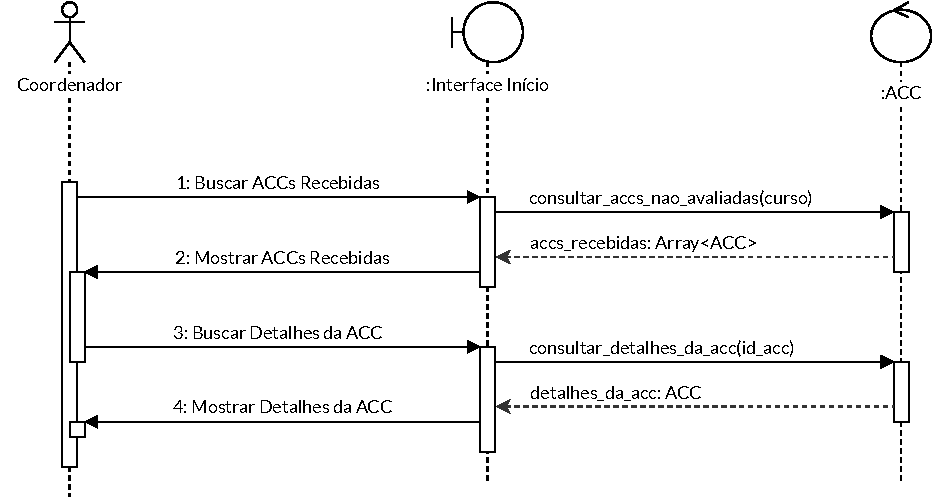
\includegraphics[width=\textwidth]{dados/figuras/Proposta/DiagramasDeSequencia/Consultar ACC.pdf}
    \caption{Diagrama de Sequência: Consultar ACC.}
    \label{diagSeq:coordConsultarACC}
\end{figure}

A Figura \ref{diagSeq:avaliarRequisicaoACC} representa a sequência das ações descritas na Tabela \ref{casoExpandido:avaliarACCs}. Esse fluxo mostra a sequência de eventos que acontecem no sistema ao ser realizada uma avaliação por parte de um Coordenador. O primeiro passo é a busca das ACCs Recebidas, realizada pelo Coordenador através da interface; Após isso o sistema exibe as ACCs recebidas, e o Coordenador escolhe uma das ACCs para buscar os detalhes; O sistema busca essas informações através do controlador de ACCs e retorna ao Coordenador através da interface; O quinto passo é a Avaliação da ACC, a partir dessa avaliação o sistema chama o controlador ACC que por sua vez chama um método para si mesmo para atualizar o \textit{status} da ACC para aprovada ou reprovada, dependendo da avaliação, e salva a avaliação da ACC através do método de salvamento do controlador AvaliacaoDaACC; Por último o sistema exibe ao Coodenador uma mensagem de confirmação de salvamento da avaliação.

\begin{figure}[H]
    \centering
    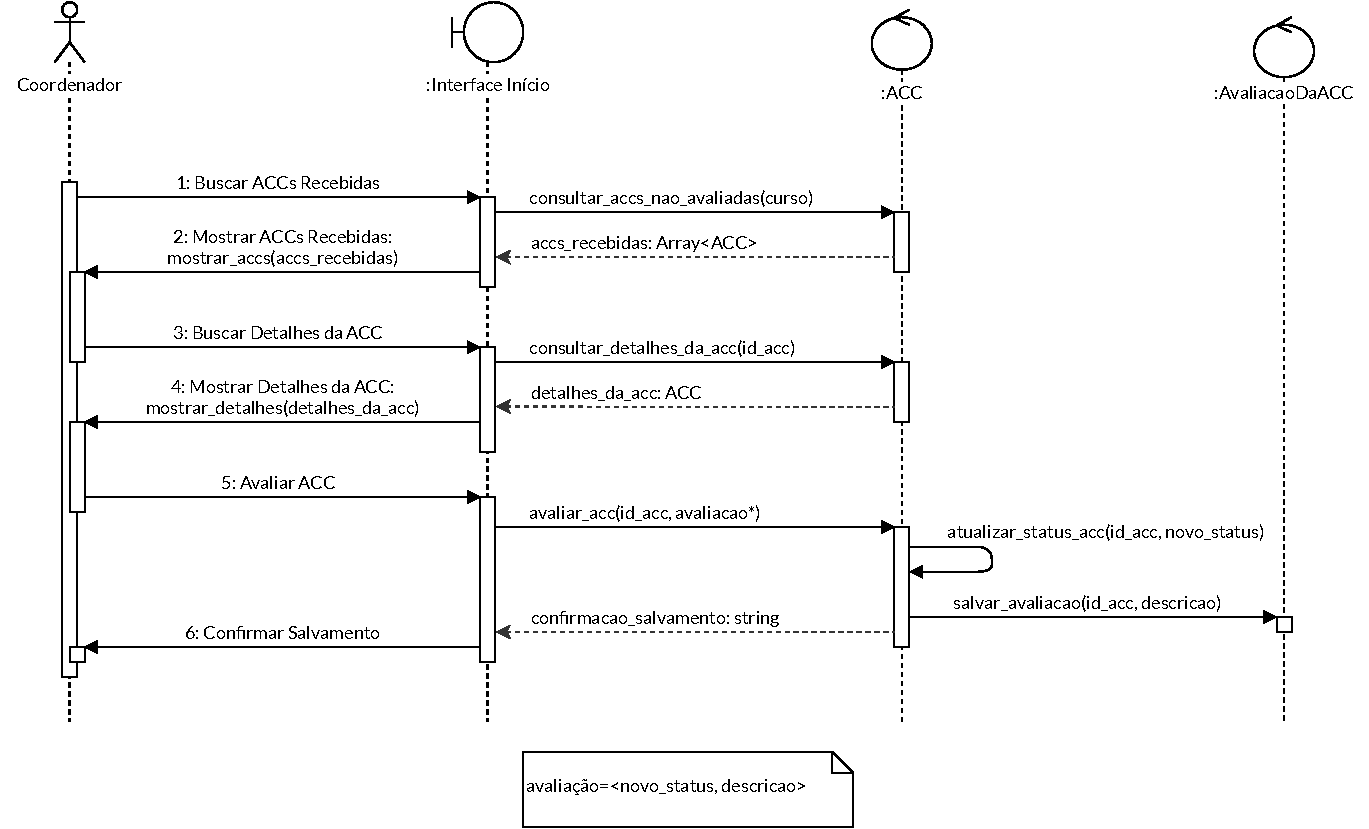
\includegraphics[width=\textwidth]{dados/figuras/Proposta/DiagramasDeSequencia/Avaliar Requisição de ACC.pdf}
    \caption{Diagrama de Sequência: Avaliar ACC.}
    \label{diagSeq:avaliarRequisicaoACC}
\end{figure}

A Figura \ref{diagSeq:consultarDiscente} representa a sequência das ações descritas na Tabela \ref{casoExpandido:consultarDiscentes}, que são realizadas por um Coordenador ao fazer a consulta dos detalhes de um Discente. O Coordenador faz a consulta dos Discentes passando como parâmetro um campo de busca através da tela de Pesquisar Discente; O sistema então faz a consulta dos Discentes através do controlador Usuario e retorna os Discentes encontrados com o parâmetro, e que estão vinculados ao mesmo curso do Coordenador, de volta para a interface, que por sua vez faz a exibição dos Discentes; A partir disso o Coordenador escolhe um dos Discentes, e consulta os seus detalhes; O sistema então faz a busca dos detalhes do Discente usando o controlador Usuario; O controlador retorna os detalhes, que por sua vez são exibidos pela interface ao Coordenador.

\begin{figure}[H]
    \centering
    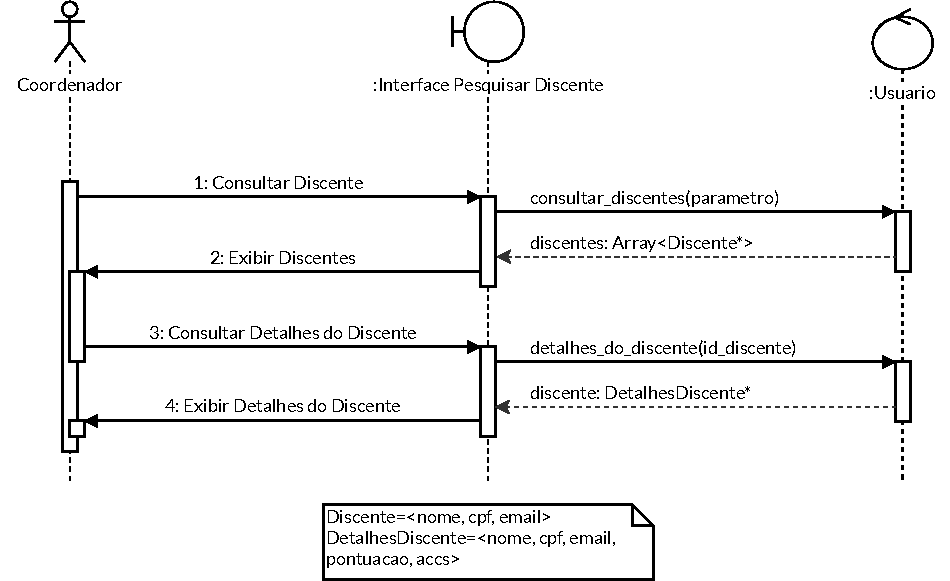
\includegraphics[width=\textwidth]{dados/figuras/Proposta/DiagramasDeSequencia/Consultar Discente.pdf}
    \caption{Diagrama de Sequência: Consultar Discente.}
    \label{diagSeq:consultarDiscente}
\end{figure}

% Discente -------------------------------------

A Figura \ref{diagSeq:consultarPontuacao} representa a sequência das ações descritas na Tabela \ref{casoExpandido:consultarPontuacao}. O diagrama demonstra o fluxo das ações de consulta da pontuação de um Discente. Primeiramente, o Discente busca a sua pontuação através da interface, após isso, o sistema envia o pedido ao controlador ACC, que calcula a pontuação de ACCs através das ACCs do Discente; Após isso o sistema retorna os resultados através da interface, exibindo na tela os pontos aprovados, em análise e reprovados do Discente.

\begin{figure}[H]
    \centering
    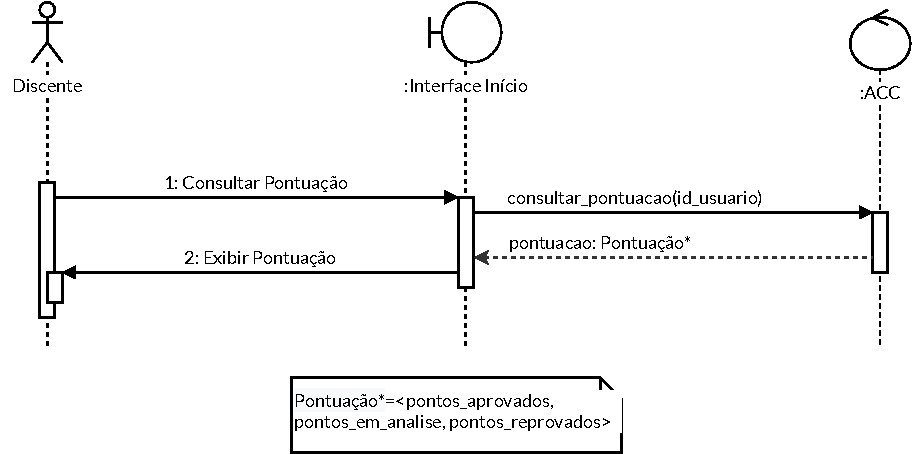
\includegraphics[width=\textwidth]{dados/figuras/Proposta/DiagramasDeSequencia/Consultar Pontuação.pdf}
    \caption{Diagrama de Sequência: Consultar Pontuação.}
    \label{diagSeq:consultarPontuacao}
\end{figure}

A Figura \ref{diagSeq:consultarTiposDeACC} representa a sequência das ações descritas na Tabela \ref{casoExpandido:consultarTiposDeACC}, que está relacionada à ação de um usuário do tipo Discente de consultar os Tipos de ACC presentes no sistema. Primeiramente, o Discente consulta os Tipos de ACC através da interface; Após isso, o sistema envia o pedido ao controlador TiposDeACC; O controlador retorna os Tipos de ACC para a interface, que por sua vez exibe para o Discente.

\begin{figure}[H]
    \centering 
    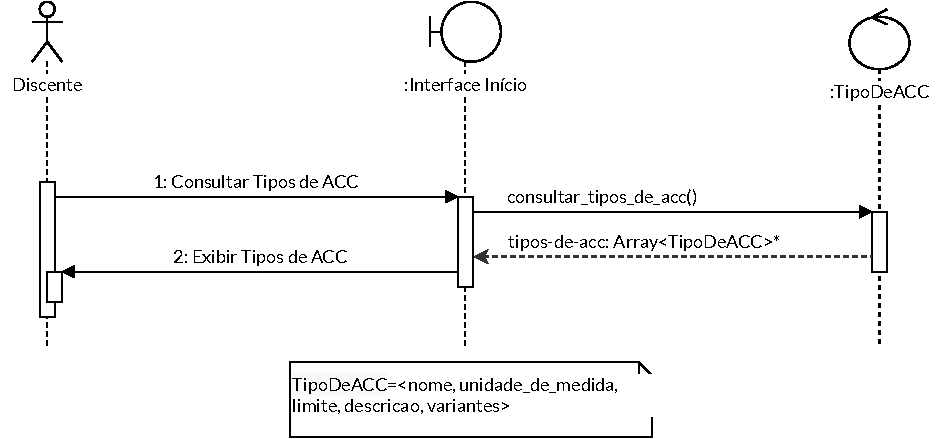
\includegraphics[width=\textwidth]{dados/figuras/Proposta/DiagramasDeSequencia/Consultar Tipos de ACC.pdf}
    \caption{Diagrama de Sequência: Consultar Tipos de ACC}
    \label{diagSeq:consultarTiposDeACC}
\end{figure}


A Figura \ref{diagSeq:gerenciarACCs} representa a sequência das ações descritas na Tabela \ref{casoExpandido:gerenciarACCs}. Esse diagrama sequencial representa as principais ações que um usuário do tipo Discente poderá realizar em relação às ACCs. A primeira etapa que o Discente realizará é a de abrir a Tela de Gerenciamento de ACCs a partir da Tela de Início; O sistema então buscará as ACCs pelo id do Discente e retornará essas ACCs à interface que fará a exibição dos dados; O Discente então escolhe uma ação entre: Cadastrar, Consultar, Editar ou Excluir; 

A partir disso o diagrama foi separado através da notação \textit{opt}, que descreve escolhas dentro de uma sequência. Essas escolhas possuem dentro de si referências, criadas através da notação \textit{ref}. Como pode ser observado na Figura \ref{diagSeq:gerenciarACCs}, há 4 \textit{opts}, sendo que cada um destes possui uma referência à outro diagrama de sequência, sendo estas: opt1 descrita na Figura \ref{diagSeq:cadastrarACC}; opt2, referenciando a Figura \ref{diagSeq:consultarACC}; opt3, como referência para a Figura \ref{diagSeq:editarACC}; e opt4 que se relaciona com a Figura \ref{diagSeq:excluirACC}.

\begin{figure}[H]
    \centering 
    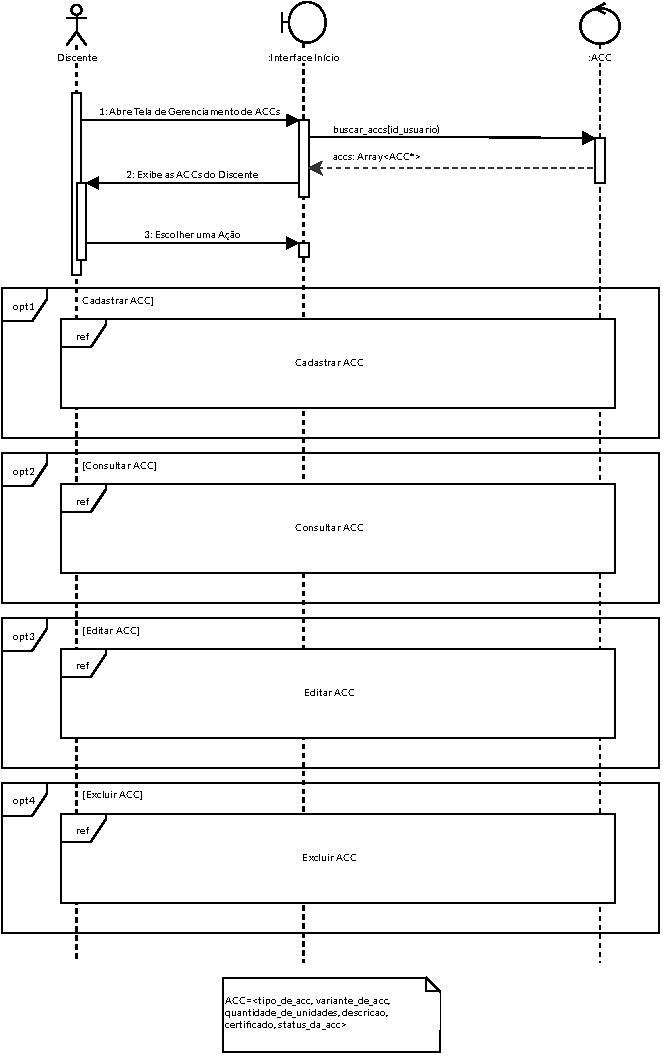
\includegraphics[width=0.8\textwidth]{dados/figuras/Proposta/DiagramasDeSequencia/Gerenciar ACCs_ Completo-Completo.pdf}
    \caption{Diagrama de Sequência: Gerenciar ACCs}
    \label{diagSeq:gerenciarACCs}
\end{figure}

A Figura \ref{diagSeq:cadastrarACC} demonstra a sequência de ações realizadas dentro do caso de uso de Cadastrar uma ACC, realizado por um Discente. Esse ação está presente no diagrama de sequência da Figura \ref{diagSeq:gerenciarACCs}. Conforme mostrado no diagrama, o Discente primeiro cadastra uma nova ACC através da tela de Cadastrar ACC preenchendo os campos necessários; Após isso o sistema faz a chamada o método de cadastro de ACC para o controlador ACC, que por sua vez retorna a confirmação de cadastro; A interface então recebe a mensagem de confirmação de cadastro e faz sua exibição.

\begin{figure}[H]
    \centering 
    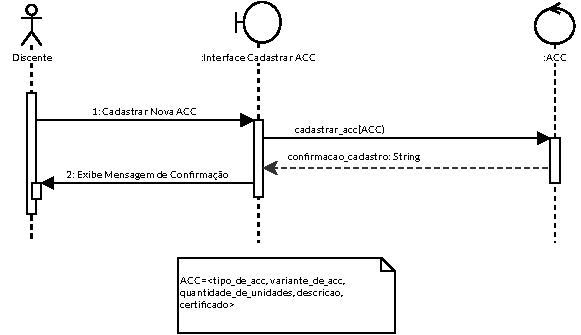
\includegraphics[width=\textwidth]{dados/figuras/Proposta/DiagramasDeSequencia/Gerenciar ACCs_ Completo-Cadastrar ACC.pdf}
    \caption{Diagrama de Sequência: Cadastrar ACC}
    \label{diagSeq:cadastrarACC}
\end{figure}

A Figura \ref{diagSeq:consultarACC} demonstra a sequência de ações realizadas pela ação de Consultar uma ACC, referenciada pelo diagrama de sequência da Figura \ref{diagSeq:gerenciarACCs}. Como mostrado no gráfico, o Discente Busca os detalhes de uma ACC através da tela de Consultar ACC; o sistema então faz a chamada do método de busca dos detalhes da ACC através do id; após isso, são retornados os detalhes da ACC selecionada, que são posteriormente exibidos ao Discente pela interface gráfica.

\begin{figure}[H]
    \centering 
    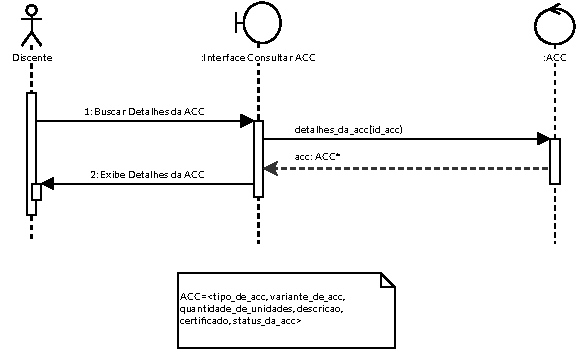
\includegraphics[width=\textwidth]{dados/figuras/Proposta/DiagramasDeSequencia/Gerenciar ACCs_ Completo-Consultar ACC.pdf}
    \caption{Diagrama de Sequência: Consultar ACC}
    \label{diagSeq:consultarACC}
\end{figure}

A Figura \ref{diagSeq:editarACC} mostra o diagrama de sequência relativo à Edição de uma ACC. Esse fluxo é referenciado pelo diagrama de sequência da Figura \ref{diagSeq:gerenciarACCs}. Como é mostrado na figura, o Discente primeiramente busca os detalhes da ACC desejada; O sistema então faz a busca pelo controlador de ACC, e retorna a ACC encontrada à interface que faz a exibição dos dados; O Discente então faz a edição dos campos através da tela de Editar ACC e envia suas alterações; O sistema por sua vez, encaminha essas alterações ao controlador, que faz o salvamento dessas edições e retorna uma mensagem de confirmação; o sistema então exibe uma mensagem de confirmação de edição ao Discente.

\begin{figure}[H]
    \centering 
    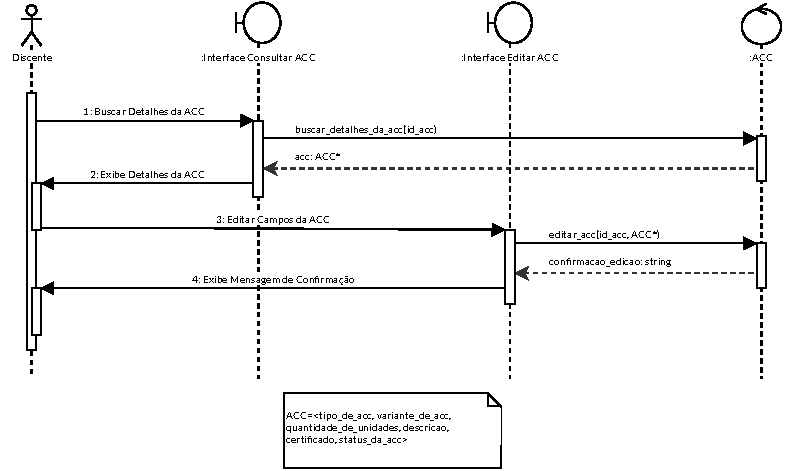
\includegraphics[width=\textwidth]{dados/figuras/Proposta/DiagramasDeSequencia/Gerenciar ACCs_ Completo-Editar ACC.pdf}
    \caption{Diagrama de Sequência: Editar ACC}
    \label{diagSeq:editarACC}
\end{figure}

A Figura \ref{diagSeq:excluirACC} mostra o diagrama de sequência relativo à Exclusão de uma ACC. Esse fluxo é referenciado pelo diagrama de sequência da Figura \ref{diagSeq:gerenciarACCs}. Como é mostrado na figura, o Discente primeiramente busca os detalhes da ACC desejada; O sistema então faz a busca pelo controlador de ACC, e retorna a ACC encontrada à interface que faz a exibição dos dados; O Discente então escolhe a opção de Excluir ACC através da tela de Consultar ACC; Após isso, o sistema faz a chamada da função de Excluir ACC do controlador de ACC; o controlador então envia uma mensagem de confirmação de exclusão, que por sua vez é mostrada ao Discente através da interface.

\begin{figure}[H]
    \centering 
    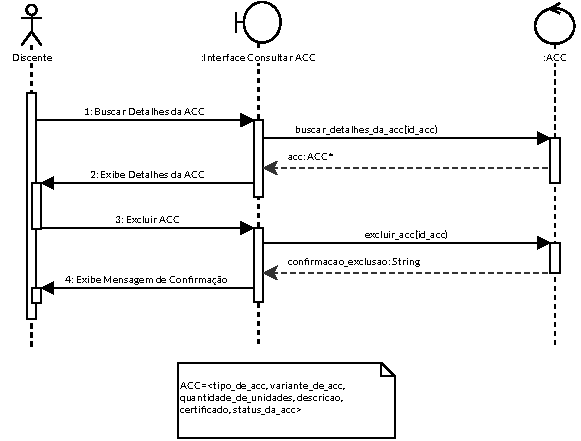
\includegraphics[width=\textwidth]{dados/figuras/Proposta/DiagramasDeSequencia/Gerenciar ACCs_ Completo-Excluir ACC.pdf}
    \caption{Diagrama de Sequência: Excluir ACC}
    \label{diagSeq:excluirACC}
\end{figure}

% Administrador -------------------------------------

O diagrama de sequência mostrado na Figura \ref{diagSeq:gerenciarTiposDeACC} diz respeito ao caso de uso expandido descrito na Tabela \ref{casoExpandido:gerenciarTiposDeACC}. Essa sequência descreve as ações de Cadastro, Atualização, Consulta e Exclusão dos Tipos de ACC presentes no sistema e que podem ser realizadas por um usuário do tipo Administrador. O Administrador primeiramente abre a tela de Gerenciamento de Tipos de ACC através da tela de Início; O sistema então faz a chamada do método de busca dos Tipos de ACC presentes no sistema através do controlador TipoDeACC; O sistema então retorna esses dados à interface que por sua vez exibe ao Administrador; O Administrador então escolhe uma das ações entre: Cadastrar, Consultar, Editar ou Excluir; A partir disso, o sistema redireciona o Administrador para as a tela da ação escolhida. Como pode ser visto na Figura \ref{diagSeq:gerenciarTiposDeACC} as ações foram divididas através de notações \textit{opt}, que por sua vez contém as referências das ações. A opt1 refere-se ao diagrama presente na Figura \ref{diagSeq:cadastrarTipoDeACC}; Já a opt2 referencia a Figura \ref{diagSeq:consultarTipoDeACC}; A opt3 por sua vez faz referência à Figura \ref{diagSeq:editarTipoDeACC}; E por último a opt4 está ligada à Figura \ref{diagSeq:excluirTipoDeACC}.

\begin{figure}[H]
    \centering
    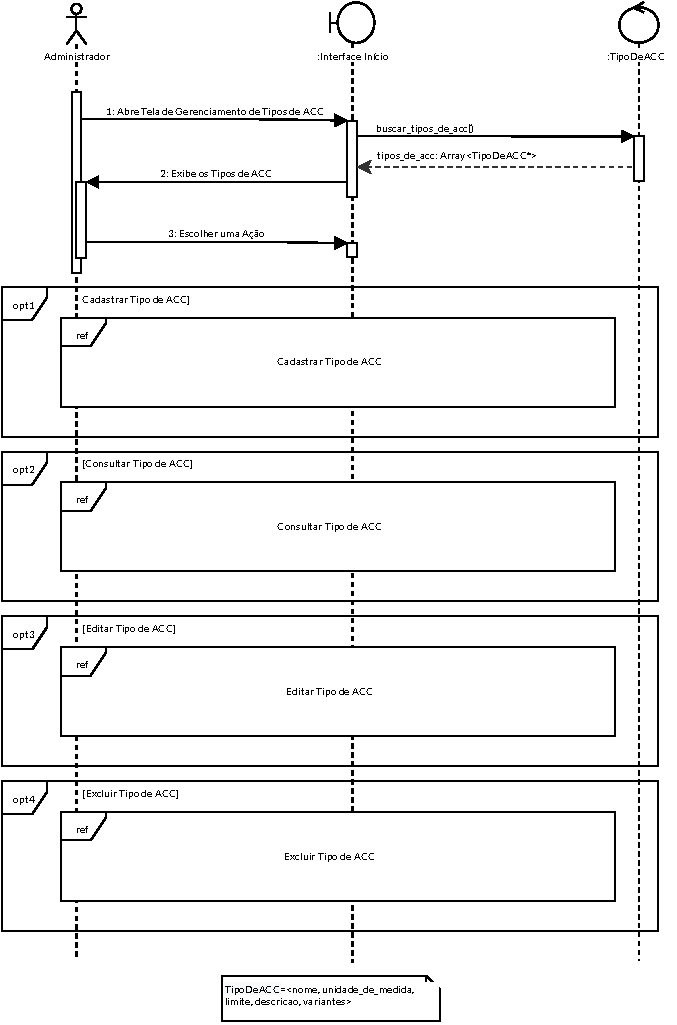
\includegraphics[width=0.8\textwidth]{dados/figuras/Proposta/DiagramasDeSequencia/Gerenciar Tipos de ACC-Completo.pdf}
    \caption{Diagrama de Sequência: Gerenciar Tipos de ACC}
    \label{diagSeq:gerenciarTiposDeACC}
\end{figure}

A Figura \ref{diagSeq:cadastrarTipoDeACC} engloba a sequência de eventos que acontecem no cadastro de um Tipo de ACC, o diagrama refere-se a uma das ações contidas dentro da Figura \ref{diagSeq:gerenciarTiposDeACC}. O Administrador do sistema faz o cadastro do Tipo de ACC preenchendo os campos necessários através da tela de Cadastrar Tipo de ACC; A interface por sua vez faz a chamada do método de cadastro de Tipo de ACC através do controlador TipoDeACC; Após isso, o controlador envia uma mensagem de confirmação de cadastro à interface, que por sua vez à exibe ao Administrador.

\begin{figure}[H]
    \centering
    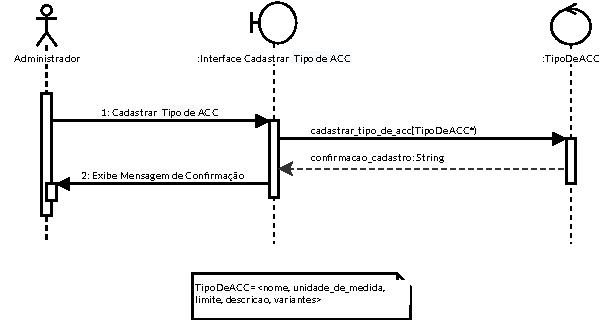
\includegraphics[width=\textwidth]{dados/figuras/Proposta/DiagramasDeSequencia/Gerenciar Tipos de ACC-Cadastrar Tipo de ACC.pdf}
    \caption{Diagrama de Sequência: Cadastrar Tipo de ACC}
    \label{diagSeq:cadastrarTipoDeACC}
\end{figure}

O diagrama descrito na Figura \ref{diagSeq:consultarTipoDeACC} é uma referência à ação de Consultar Tipo de ACC, presente no diagrama mostrado na Figura \ref{diagSeq:gerenciarTiposDeACC}. O consultor primeiramente realiza a busca dos detalhes de um Tipo de ACC, através da interface gráfica; O sistema por sua vez faz a chamada do método que faz a consulta dos detalhes de um Tipo de ACC; A partir disso, o controlador retorna esses dados à interface que por sua vez faz a exibição ao Administrador.

\begin{figure}[H]
    \centering
    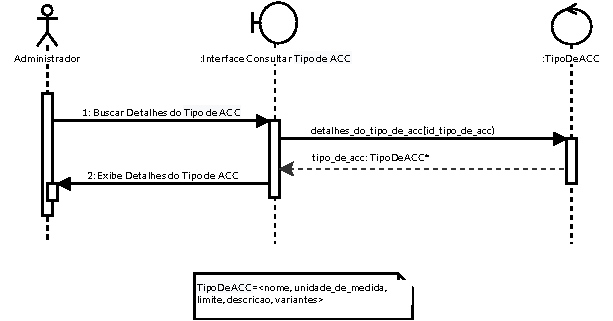
\includegraphics[width=\textwidth]{dados/figuras/Proposta/DiagramasDeSequencia/Gerenciar Tipos de ACC-Consultar Tipo de ACC.pdf}
    \caption{Diagrama de Sequência: Consultar Tipo de ACC}
    \label{diagSeq:consultarTipoDeACC}
\end{figure}

A ação de Editar Tipo de ACC, presente no diagrama da Figura \ref{diagSeq:gerenciarTiposDeACC} está descrito na Figura \ref{diagSeq:editarTipoDeACC}. O Administrador primeiramente faz a consulta dos detalhes do Tipo de ACC através da tela de Consultar Tipo de ACC; O sistema por sua vez chama a função de buscar detalhes do Tipo de ACC presente no controlador TipoDeACC; O controlador por sua vez, retorna os dados do Tipo de ACC que são então retornados ao Administrador através da interface gráfica; O Administrador então faz o preenchimento das alterações necessárias no Tipo de ACC através da tela de Editar Tipo de ACC e submete essas alterações; A interface envia essas alterações para serem salvas pelo controlador; O controlador então retorna uma mensagem de confirmação da edição, que por sua vez é exibida ao Administrador através da interface.

\begin{figure}[H]
    \centering
    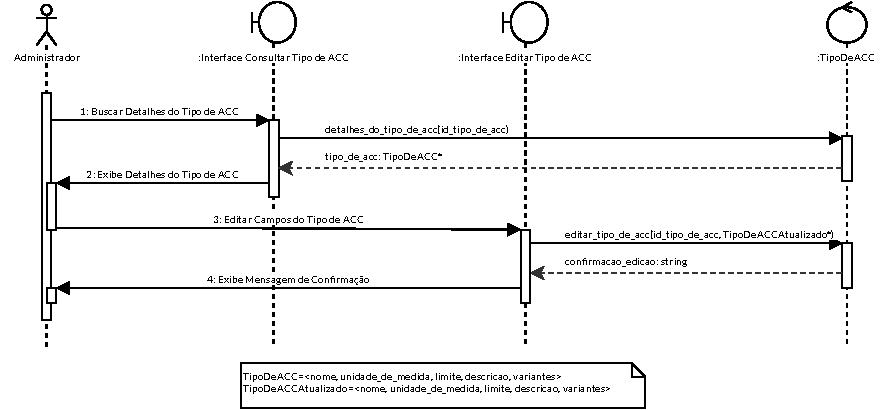
\includegraphics[width=\textwidth]{dados/figuras/Proposta/DiagramasDeSequencia/Gerenciar Tipos de ACC-Atualizar Coordenador.pdf}
    \caption{Diagrama de Sequência: Editar Tipo de ACC}
    \label{diagSeq:editarTipoDeACC}
\end{figure}

A Figura \ref{diagSeq:excluirTipoDeACC} demonstra o diagrama de sequência correspondente à ação de Excluir Tipo de ACC, presente no diagrama encontrado na Figura \ref{diagSeq:gerenciarTiposDeACC}, e descreve a sequência de eventos que acontecem durante a exclusão de um Tipo de ACC realizada por um Administrador. O Administrador faz a busca dos Detalhes do Tipo de ACC através da interface, esta faz a chamada do método de consulta dos detalhes de um Tipo de ACC presente no controlador TipoDeACC; O controlador retorna os dados do Tipo de ACC à interface que por sua vez exibe ao Administrador; O Administrador então escolhe a opção de Excluir Tipo de ACC; A partiri disso, o sistema faz a exclusão do Tipo de ACC utilizando o identificador único do Tipo de ACC; O controlador então envia uma mensagem de confirmação da exclusão, que é então exibida ao Administrador pela interface.

\begin{figure}[H]
    \centering
    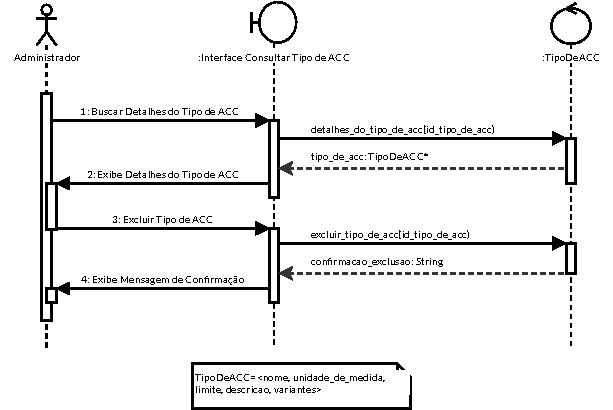
\includegraphics[width=\textwidth]{dados/figuras/Proposta/DiagramasDeSequencia/Gerenciar Tipos de ACC-Excluir Tipo de ACC.pdf}
    \caption{Diagrama de Sequência: Excluir Tipo de ACC}
    \label{diagSeq:excluirTipoDeACC}
\end{figure}

O diagrama de sequência mostrado na Figura \ref{diagSeq:gerenciarCoordenadores} diz respeito ao caso de uso expandido descrito na Tabela \ref{casoExpandido:gerenciarCoordenadores}, e mostra o gerenciamento de coordenadores, ação realizada por um usuário do tipo Administrador. Conforme o diagrama, a primeira ação que o Administrador realiza é a de abrir a tela de gerenciamento de Coordenadores através da tela Inicial; Após isso, o sistema busca os usuários do tipo Coordenador presentes no sistema através do controlador Usuario; Após isso, o controlador retorna os Coordenadores encontrados à interface que por sua vez renderiza a lista recebida; O Administrador então escolhe uma ação entre: Cadastrar, Consultar, Editar e Excluir. Como pode ser visto na Figura \ref{diagSeq:gerenciarCoordenadores}, essas ações são divididas utilizando a notação \textit{opt}, que denota opções que podem ser escolhidas dentro de uma sequência, cada uma dessas \textit{opts} possuem uma referência para outro diagrama de sequência utilizando a notação \textit{ref}, tal estratégia foi utilizada para diminuir a complexidade do diagrama e melhorar a compreensão. As ações estão referenciadas da seguinte forma: opt1 fazendo referência à Figura \ref{diagSeq:cadastrarCoordenador}; opt2 sendo demonstrada na Figura \ref{diagSeq:consultarCoordenador}; opt3 referenciando a Figura \ref{diagSeq:editarCoordenador}; e opt4 sendo uma referência à Figura \ref{diagSeq:excluirCoordenador}.

\begin{figure}[H]
    \centering
    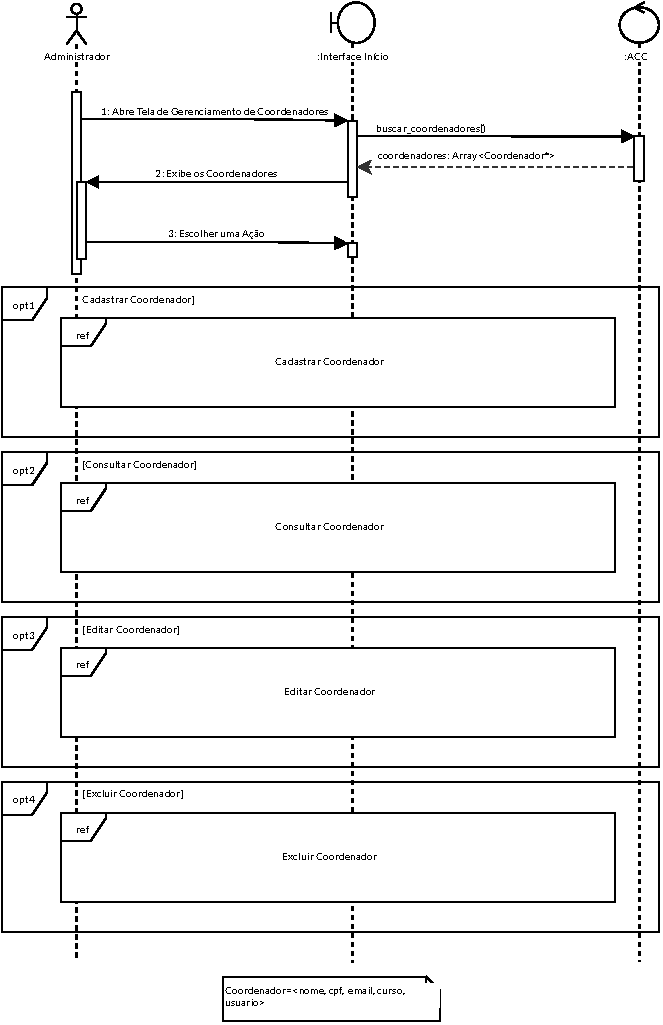
\includegraphics[width=0.8\textwidth]{dados/figuras/Proposta/DiagramasDeSequencia/Gerenciar Coodenadores-Completo}
    \caption{Diagrama de Sequência: Gerenciar Coordenadores}
    \label{diagSeq:gerenciarCoordenadores}
\end{figure}

A Figura \ref{diagSeq:cadastrarCoordenador} demonstra o diagrama de sequência referente ao cadastro de um Coordenador, presente dentro do diagrama de Gerenciamento de Coordenadores, mostrado na Figura \ref{diagSeq:gerenciarCoordenadores}. O Administrador primeiramente realiza o cadastro de um Coordenador através da tela de Cadastrar Coordenador; A interface então faz a chamada do método de cadastrar um novo usuário do tipo coordenador através do controlador Usuario; O controlador então retorna uma mensagem de confirmação de cadastro que por sua vez é exibida ao usuário através da interface.

\begin{figure}[H]
    \centering
    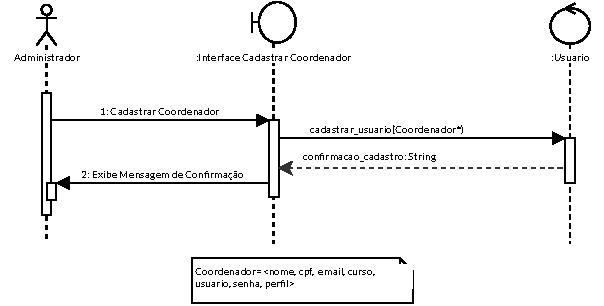
\includegraphics[width=\textwidth]{dados/figuras/Proposta/DiagramasDeSequencia/Gerenciar Coodenadores-Cadastrar Coordenador.pdf}
    \caption{Diagrama de Sequência: Cadastrar Coordenador}
    \label{diagSeq:cadastrarCoordenador}
\end{figure}

A Figura \ref{diagSeq:consultarCoordenador} mostra o diagrama de sequência referente à ação de Consultar Coordenador, presente na Figura \ref{diagSeq:gerenciarCoordenadores}, e demonstra a sequência de eventos que acontecem quando um Administrador realiza a consulta dos detalhes de um Coordenador. O Administrador escolhe um dos Coordenadores e busca os seus detalhes; A interface busca os detalhes do Coordenador através do método de consulta presente no controlador de Usuario; Após isso, o controlador retorna os dados do Coordenador à interface, que por sua vez exibe ao Administrador.

\begin{figure}[H]
    \centering
    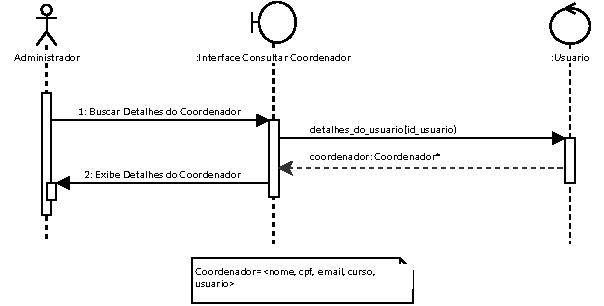
\includegraphics[width=\textwidth]{dados/figuras/Proposta/DiagramasDeSequencia/Gerenciar Coodenadores-Consultar Coordenador.pdf}
    \caption{Diagrama de Sequência: Consultar Coordenador}
    \label{diagSeq:consultarCoordenador}
\end{figure}

A Figura \ref{diagSeq:editarCoordenador} mostra o diagrama de sequência de Editar Coordenador, ação realizada por um Administrador e presente dentro do diagrama de sequência da Figura \ref{diagSeq:gerenciarCoordenadores}. A primeira ação realizada pelo Administrador é fazer a busca dos detalhes de um Coordenador através da Tela de Consultar Coordenador; O sistema faz a busca desses detalhes através do método presente no controlador de Usuario; O controlador retorna os detalhes do Discente à interface, que por sua vez exibe ao Administrador; A partir disso, o Administrador escolhe a opção de Editar Coordenador, e faz a edição dos detalhes do Coordenador através da tela de Editar Coordenador; O Administrador então submete as alterações, que são enviadas ao controlador pela interface; O controlador faz o salvamento dos dados e retorna uma mensagem de confirmação da edição que por sua vez é exibida ao Administrador pela interface gráfica.

\begin{figure}[H]
    \centering
    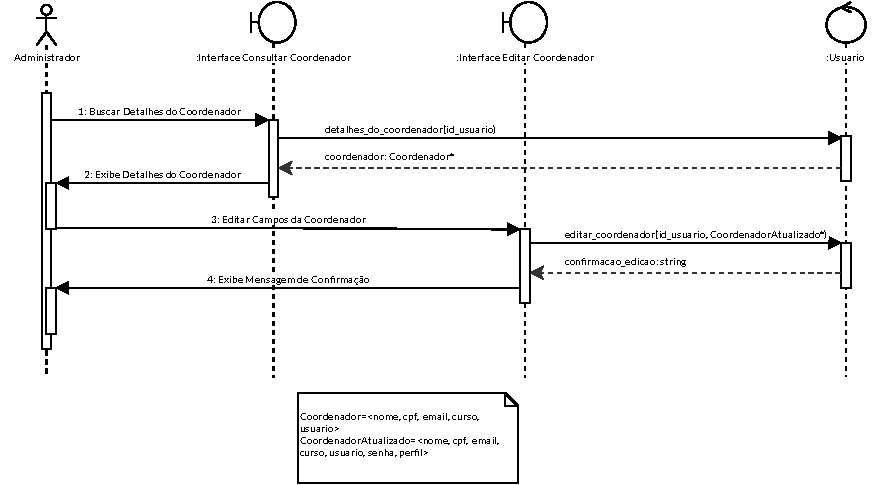
\includegraphics[width=\textwidth]{dados/figuras/Proposta/DiagramasDeSequencia/Gerenciar Coodenadores-Atualizar Coordenador.pdf}
    \caption{Diagrama de Sequência: Editar Coordenador}
    \label{diagSeq:editarCoordenador}
\end{figure}

A Figura \ref{diagSeq:excluirCoordenador} exibe o diagrama de sequência referente à ação de Excluir Coordenador, presente no diagrama de sequência exibido na Figura \ref{diagSeq:gerenciarCoordenadores}. O Administrador faz a busca dos detalhes do Coordenador, através da tela de Consultar Coordenador; O sistema faz a busca dos dados através do controlador de Usuario; O controlador então retorna os dados que são então exibidos ao Administrador através da interface gráfica; Após isso o Administrador seleciona a opção de Excluir Coordenador; O sistema realiza a exclusão do Coordenador utilizando o seu identificador único através do método presente no controlador Usuario; O controlador então retorna uma mensagem de confirmação da exclusão, que é então exibida ao Administrador através da interface gráfica.

\begin{figure}[H]
    \centering
    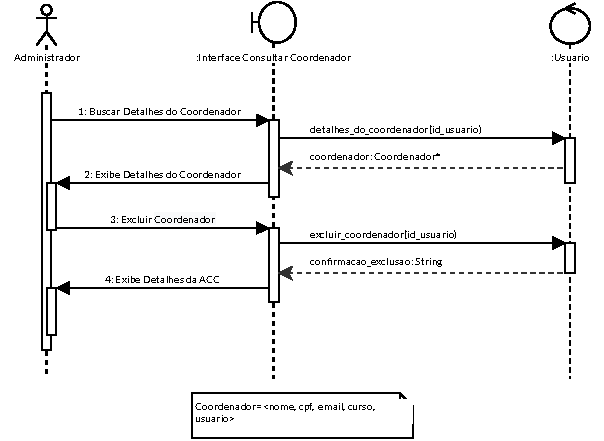
\includegraphics[width=\textwidth]{dados/figuras/Proposta/DiagramasDeSequencia/Gerenciar Coodenadores-Excluir Coordenador.pdf}
    \caption{Diagrama de Sequência: Excluir Coordenador}
    \label{diagSeq:excluirCoordenador}
\end{figure}

\subsection{Modelo Conceitual}
\label{sec:modeloConceitual}

Segundo \cite{wazlawick2014analise} o modelo conceitual descreve a informação que será gerenciada pelo sistema, mostrando uma visão de próxima à de um usuário do sistema. A Figura \ref{fig:modeloConceitual} descreve as informações manipuladas pelo sistema, sendo estas:
\begin{itemize}
    \item Curso: descreve o curso ao qual um usuário está vinculado, sendo necessário apenas o nome do mesmo. Ele se relaciona diretamente com a entidade Usuario através de uma relação de Um para Muitos, onde um curso pode possuir vários usuários, mas cada usuário pode possuir apenas um curso;
    \item Usuario: é a informação sobre o usuário que está utilizando o sistema, sendo responsável por guardar tanto os dados dos discentes, quanto dos coordenadores e administradores. Essa entidade está ligada à Enumeração Perfil, que por sua vez descreve qual o perfil do usuário cadastrado, através de uma relação de Muitos para Um, onde cada Perfil possui vários Usuarios, mas cada Usuario possui apenas um Perfil; A mesma relação de Usuario e Perfil é encontrada entre Usuario e Curso; Há ainda uma relação de Um para Muitos com a entidade ACC, e de Um para Um com Login, onde cada Usuario possui um Login e vice-versa;
    \item Login: responsável por guardar os dados de login de um usuário, bem como o seu token de acesso ao sistema. Essa informação relaciona-se de Um para Um com o Usuario, pois cada Usuario possui apenas um Login, e um Login apenas um Usuario;
    \item ACC: guarda as informações sobre a ACC de um discente. Está ligada à Enumeração StatusDaACC, que mostra qual o estado da ACC dentro do sistema (Aprovada, Reprovada ou Em análise), através de uma relação de Muitos para Um, a mesma relação se encontra com as entidades Usuario, TipoDeACC e VarianteDaACC; Já o relacionamento de ACC com Certificado é de Um para Um, onde cada ACC possui apenas um Certificado e vice-versa;
    \item Certificado: responsável por guardar os dados de um certificado vinculado a uma ACC. Relaciona-se unicamente com ACC, numa relação de Um para Um;
    \item TipoDeAcc: guarda os tipos de ACC presentes no sistema, sendo necessária a utilização da Enumeração UnidadeDeMedida, que descreve os tipos de unidade de medida do sistema (Hora, Semestre, Curso etc). Possui uma relação de Um para Muitos com ACC, onde cada TipoDeACC pode ter várias ACCs, mas cada ACC pode possuir apenas um TipoDeACC; Já sua relação com VarianteDaACC se dá em Um para Um, e com UnidadeDeMedida em Muitos para Um;
    \item VarianteDeAcc: guarda os tipos de variações de ACCs, por exemplo se uma ACC é na área dos cursos da FACEEL ou não. As variações são utilizadas para o calculo de proporção por unidade de medida do tipo de ACC que ela está associada. Relaciona-se de Um para Muitos com ACC, e de Um para Um com TipoDeACC;
    \item UnidadeDeMedida: Responsável por guardar as unidades de medida presentes nos TiposDeACC, essas unidades são Hora, Semestre, Curso, Trabalho, entre outros. Possui relação unicamente com TipoDeACC, em uma proporção de Um para Muitos;
\end{itemize}

\begin{figure}[H]
    \centering
    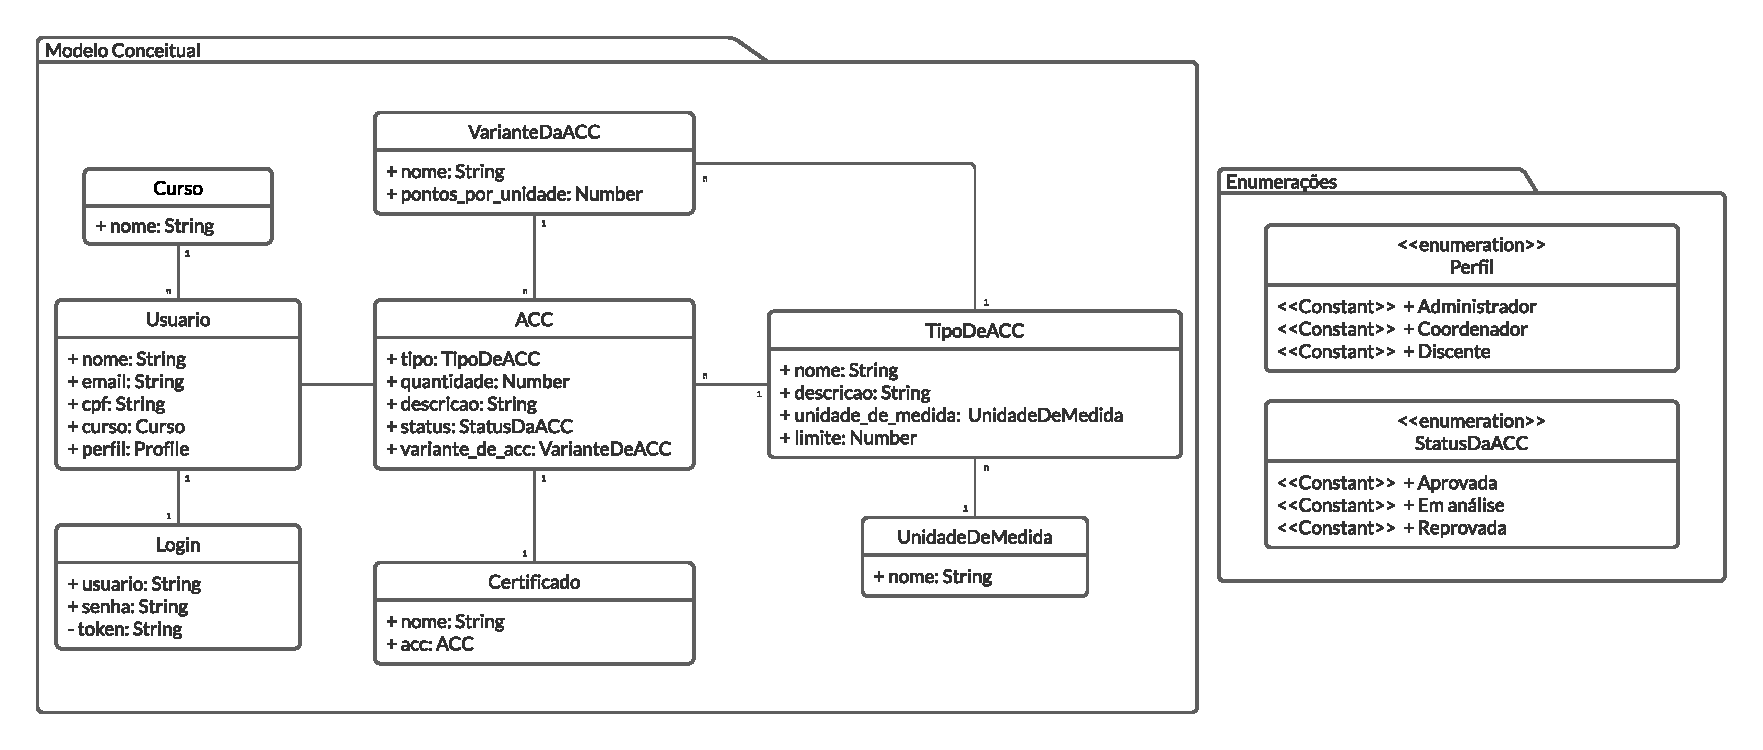
\includegraphics[width=\textwidth]{dados/figuras/Proposta/modelo_conceitual__keeme.pdf}
    \caption{Modelo Conceitual do Sistema}
    \label{fig:modeloConceitual}
\end{figure}

\subsection{Diagrama de Entidade Relacionamento}
\label{sec:diagramaER}

O Diagrama de Entidade Relacionamento, é descrito por \cite{lucid2021er} como sendo um diagrama que mostra como as entidades relacionam-se entre si dentro de um determinado sistema. São utilizados dentro da Engenharia de Software para se fazer a modelagem dos bancos de dados relacionais. A Figura \ref{fig:entidadeRelacionamento} demonstra o diagrama de entidade relacionamento referente à base de dados utilizada pela aplicação desenvolvida neste trabalho.

\begin{figure}[H]
    \centering
    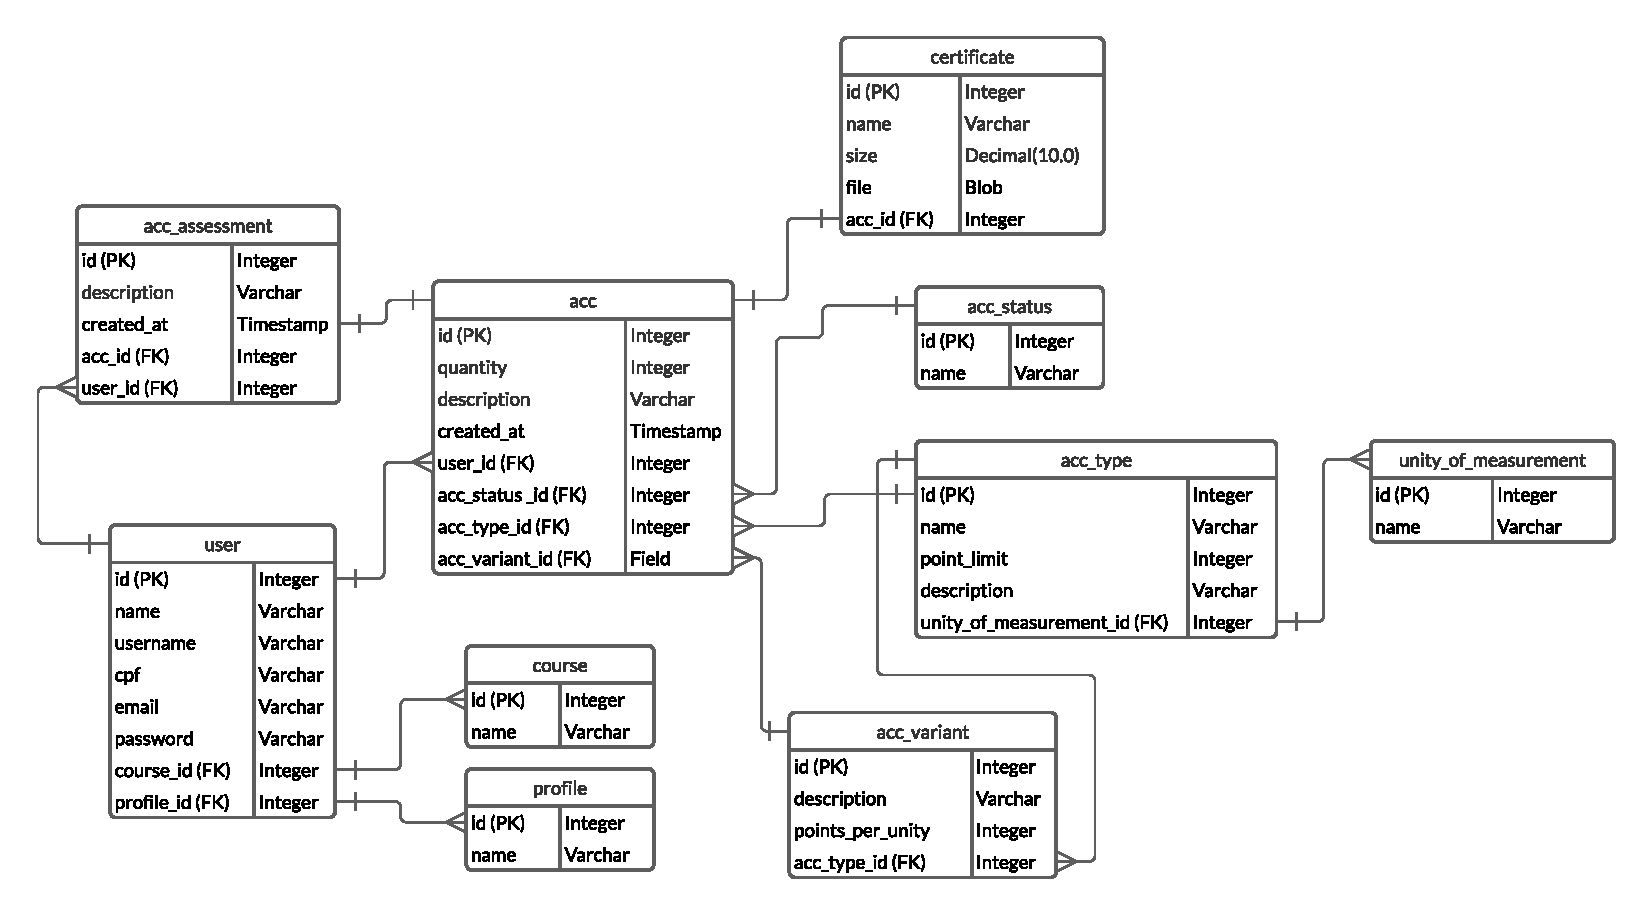
\includegraphics[width=\textwidth]{dados/figuras/Proposta/Diagrama Keep It To Me - v1.0 MVP.pdf}
    \caption{Banco de Dados da Aplicação KeeMe}
    \label{fig:entidadeRelacionamento}
\end{figure}

\begin{itemize}
    
    \item user (usuário): essa entidade armazena os dados dos usuários da aplicação. Seus campos são:
    \begin{itemize}
        \item id: identificador único do usuário;
        \item name (nome): guarda o nome do usuário;
        \item username: guarda o apelido do usuário, utilizado para a função de login na plataforma;
        \item cpf: armazena o cpf do usuário, utilizado para facilitar as funções de busca de discentes;
        \item email: campo referente ao email do usuário, utilizado para funções que envolvam confirmação de criação de perfil e recuperação de senhas;
        \item password (senha): senha que o usuário utilizará para entrar no sistema. Nesta aplicação em específico, está sendo usada a criptografia MD5 para armazenar as senhas dos usuários, e impedir a sua desencriptação;
        \item course\_id: id do curso ao qual o usuário está vinculado. Um usuário pode estar vinculado a apenas um curso;
        \item profile\_id: id do perfil do usuário no sistema. Um usuário pode ter apenas um perfil por vez;
    \end{itemize}
    
    \item course (curso): entidade responsável por armazenar os dados dos cursos presentes na base. Um curso pode ter um ou mais usuários, porém um usuário pode ter apenas um curso. Seus campos são:
    \begin{itemize}
        \item id: identificador único do curso;
        \item name (nome): nome do curso;
    \end{itemize}
    
    \item profile (perfil): responsável por guardar os perfis dos usuários no sistema, é utilizada para funções de autenticação de usuários. Um perfil pode conter um ou mais usuários, mas cada usuário pode ter apenas um perfil no sistema. Seus campos são:
    \begin{itemize}
        \item id: identificador único do perfil;
        \item name (nome): nome do perfil;
    \end{itemize}
    
    \item unity\_of\_measurement (unidade de medida): Armazena os tipos de unidade de medida presentes no sistema, esses tipos se referem a como os pontos de ACCs são contados, por exemplo: horas, semestres, certificados, etc. Seus campos são:
    \begin{itemize}
        \item id: identificador único da unidade de medida;
        \item name (nome): nome da unidade de medida;
    \end{itemize}
    
    \item acc\_type (tipo de acc): Essa entidade é responsável por guardar os dados de tipos de ACC presentes no sistema, esses tipos são as atividades presentes no regulamento de ACC, como por exemplo a realização de minicursos. Seus campos são:
    \begin{itemize}
        \item id: identificador único do tipo de ACC;
        \item name (nome): nome do tipo de ACC;
        \item point\_limit (limite de pontos): refere-se ao limite máximo de pontos que um usuário pode conseguir em determinada modalidade de ACC;
        \item description (descrição): guarda o detalhamento daquilo que a ACC se refere, sendo um campo adicional para facilitar o entendimento por parte dos discentes;
        \item unity\_of\_measurement\_id: identificador da unidade de medida do tipo de ACC.
    \end{itemize}
    
    \item acc\_variant (variante da acc): esta classe guarda as variantes de ACC presentes no sistema. Variantes são subtipos de ACCs, elas foram criadas por conta da existência de tipos de ACC que possuem mais de um tipo de estratégia de pontuação, mas que essas estratégias estão sob o mesmo limite de pontuação. Seus campos são:
    \begin{itemize}
        \item id: identificador único da variante de acc;
        \item description (descrição): uma descrição do que a variante se refere, por exemplo, minicurso na área dos cursos da FACEEL;
        \item points\_per\_unity (pontos por unidade): esse campo refere-se à quantidade de pontos que um usuário pode obter por unidade de medida do tipo de ACC. Por exemplo, um discente poderá obter 6 pontos por semestre em um estágio não obrigatório, onde os pontos por unidade nesse caso são 6, e a unidade de medida é Semestre;
        \item acc\_type\_id: tipo de ACC ao qual a variante está associada;
    \end{itemize}
    
    \item acc\_status (status da acc): refere-se aos status que as accs estão dentro do sistema, são status como aprovada ou reprovada. Seus campos são:
    \begin{itemize}
        \item id: identificador único do status da ACC;
        \item quantity (nome): nome do status da ACC;
    \end{itemize}

    \item acc: é a classe central do sistema, responsável por guardar as informações sobre as ACCs obtidas pelos discentes do sistema. Seus campos são:
    \begin{itemize}
        \item id: identificador único da ACC;
        \item quantity (quantidade): a quantidade refere-se diretamente à unidade de medida do tipo de ACC ao qual a ACC está associada. Sendo que essa quantidade é o número de horas, semestres, certificados, etc, que o usuário possui naquela ACC;
        \item created\_at (criada em): guarda o momento da criação da ACC;
        \item user\_id (id do usuário): associa a ACC a um usuário presente no sistema;
        \item acc\_status\_id (status da acc): armazena o status da ACC através de uma chave estrangeira;
        \item acc\_type (tipo de acc): referencia o tipo da ACC;
        \item acc\_variant\_id (id da variante de acc): relaciona a ACC a uma variante do sistema;
    \end{itemize}
    
    \item acc\_assessment (avaliação da acc): salva as informações de uma avaliação de ACC realizada por um Coordenador do sistema. Seus campos são:
    \begin{itemize}
        \item id: identificador único da avaliação de ACC;
        \item created\_at (criada em): data da avaliação de ACC;
        \item description (descrição): Motivo pelo qual uma ACC foi reprovada, esse campo só é usado em caso de reprovações;
        \item user\_id (id do usuário): relaciona o coordenador responsável pela avaliação da ACC;
    \end{itemize}
\end{itemize}

\section{Arquitetura do Sistema KeeMe}
\label{sec:arquiteturaDoSistema}

Foi utilizada uma arquitetura baseada em microserviços na aplicação, onde há um servidor \textit{Back-end} que é responsável pela lógica da aplicação, e pelas regras de negócio, e um servidor \textit{Front-end}, cujo intuito e a visualização dos dados e interação com a ferramenta.

A Figura \ref{fig:arquiteturaKeeme} demonstra de maneira visual a arquitetura utilizada na ferramenta KeeMe. O servidor \textit{Back-end} da aplicação é responsável por toda parte lógica da aplicação, como a calculo de pontos dos alunos, e por todas as funções de manipulação da base de dados, sendo que a utilização de suas funções são feitas através dos serviços que ele provê, que são chamados através das rotas providas pelo mesmo. O servidor \textit{Front-end} tem como única responsabilidade prover uma interface de utilização do sistema, desta forma, não possui nenhuma regra de negócio, mas apenas consome os serviços providos pelo \textit{Back-end}, em outras palavras, o \textit{Front-end} não faz nenhuma interação direta com a base de dados. Os clientes por sua vez consomem o \textit{Front-end} através de computadores, celulares ou tablets, e interagem com o sistema através dele, dessa forma os clientes não podem interagir diretamente com o \textit{Back-end} ou com a base, mas apenas com o \textit{Front-end}

\begin{figure}[H]
    \centering
    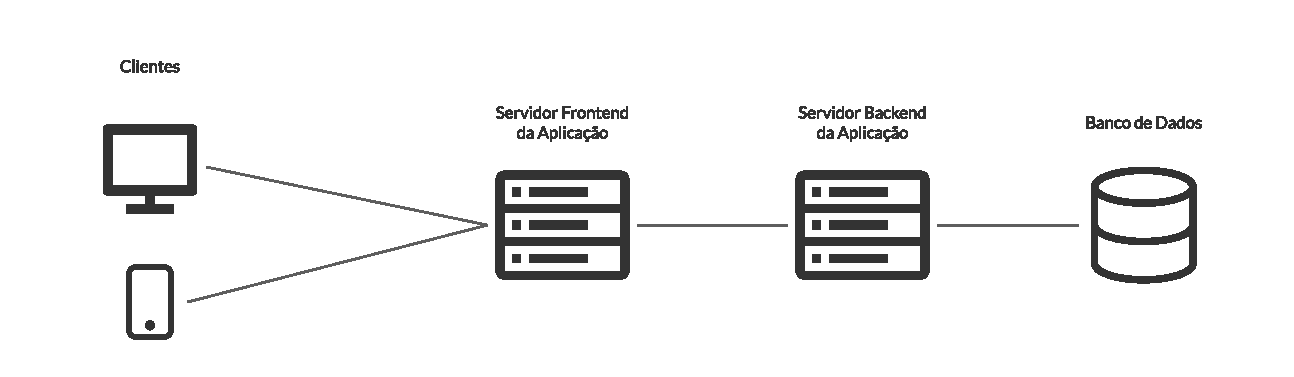
\includegraphics[width=\textwidth]{dados/figuras/Proposta/arquitetura_keeme.pdf}
    \caption{Arquitetura do Sistema KeeMe.}
    \label{fig:arquiteturaKeeme}
\end{figure}

A estratégia de dividir as responsabilidades em microserviços foi utilizada primeiramente pela melhoria na manutenibilidade do sistema, separando a parte visual da parte lógica, e também como forma de desacoplar a lógica do sistema, tornando-a independente, e assim caso haja a necessidade de se refazer o \textit{Front-end}, ou mesmo de criar uma aplicação voltada para dispositivos móveis ou computadores, não é necessário reimplementar a lógica, mas apenas consumir os serviços já providos pelo \textit{Back-end}.

\section{Implementação do KeeMe}
\label{sec:implementacao}

A implementação da aplicação foi feita utilizando o Typescript tanto no \textit{Back-end} quanto no \textit{Front-end}, que por sua vez foi feito utilizando como base a biblioteca React. O desenvolvimento da interface foi feito buscando uma solução que fosse amigável, minimalista, mas que possuísse todas as informações relevantes aos discentes.

\subsection{\textit{Back-end}}

O \textit{Back-end} da aplicação foi criado utilizando o Typescript, implementando um servidor REST, que segundo \cite{costa2020__rest} deve ser visto como um modelo de comunicação entre sistemas distribuídos, no qual o \textit{Front-end} e o \textit{Back-end} são criados sem interferência um com o outro, dessa forma o servidor do KeeMe é responsável por prover os serviços através das rotas presentes nele. Como explicado na subseção \ref{sec:arquiteturaDoSistema} o \textit{Back-end} do KeeMe funciona como a parte lógica do sistema, além de fazer as operações com a base de dados.

A Arquitetura do \textit{Back-end} foi feito utilizando o SOLID, que por usa fez consiste em princípios da Programação Orientada a Objetos que facilitam o desenvolvimento e a manutenção de aplicações. Segundo \cite{paixao2020__solid} o SOLID é uma sigla para os seguintes princípios: 

\begin{itemize}
    \item S — Single Responsiblity Principle (Princípio da responsabilidade única)
    \item O — Open-Closed Principle (Princípio Aberto-Fechado)
    \item L — Liskov Substitution Principle (Princípio da substituição de Liskov)
    \item I — Interface Segregation Principle (Princípio da Segregação da Interface)
    \item D — Dependency Inversion Principle (Princípio da inversão da dependência)
\end{itemize}

O Princípio da responsabilidade única, de acordo com \cite{paixao2020__solid}, descreve que cada classe deve possuir apenas uma única responsabilidade dentro do sistema. Durante o desenvolvimento de uma aplicação, há a tendencia de se agrupar todas as funções de uma determinada entidade sobre a mesma classe, como as ações de criação, consulta, edição e exclusão, e por mais que seja eficiente a primeiro momento, quando o número de métodos na classe começa a crescer a complexidade das mesmas também cresce, torna cada vez mais complicado realizar mudanças. Ao dar cada classe uma única responsabilidade, se torna mais simples a manutenção do código, e os impactos das mudanças tornam-se mais rastreáveis.

O Princípio Aberto-Fechado defende que todas as classes devem estar abertas para extensão, porém fechadas para edição. Um dos grandes causadores de erros em sistemas, é a mudança da lógica de métodos e classes que estão funcionando corretamente. Por conta disso, este princípio descreve que caso seja necessário fazer uma operação diferente com o mesmo método, é preferível criar outra método, ou uma classe separada para isso, deixando as classes já funcionais imutáveis.

O Princípio da substituição de Liskov, segundo \cite{paixao2020__solid}, defende que uma classe filha deve ser substituível por sua classe pai sem que seja necessário alterar as propriedades do programa. A aplicação deve ser desenvolvida de forma que suas abstrações possam permitir esse princípio.

O Princípio da segregação de interface por sua vez explica que as classes não devem implementar métodos que não irão ser utilizados. Dessa forma, é preferível criar interfaces mais específicas do que uma interface genérica que englobe todos os métodos \cite{paixao2020__solid}.

E por último, o Princípio da inversão de dependência defende a dependência de abstrações ao invés de implementações \cite{paixao2020__solid}. Em outras palavras, ao invés de se fazer a implementação de uma dependência dentro da classe, é preferível que essa dependência seja recebida como uma abstração pelo construtor, e este faça o instanciamento da dependência em tempo de execução.

Além dos princípios do SOLID foram usadas também estratégias de autenticação dos serviços providos pelo \textit{Back-end} usando JWT (JSON Web Token). A Figura \ref{fig:codigoGeradorDeToken} mostrará a função responsável pela geração dos tokens JWT, a função recebe o id do usuário e o perfil do mesmo, e a partir disso faz a geração de um token único vinculado ao login feito.

\begin{figure}[H]
    \centering
    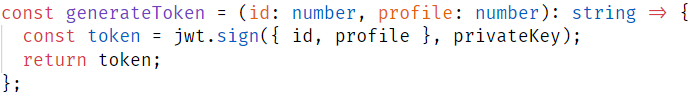
\includegraphics[width=0.80\textwidth]{dados/figuras/Proposta/Códigos/code_generate_token.png}
    \caption{Geração de Tokens usando JWT}
    \label{fig:codigoGeradorDeToken}
\end{figure}

A Figura \ref{fig:codigoValidadorDeToken} mostra a validação dos tokens recebidos. A função de validação funciona como um \textit{middleware} que recebe os dados da requisição recebidos por um consumidor, e tenta encontrar o Token no Header da requisição. Caso encontre o token, e o mesmo seja válido, o sistema continua a operação. Caso o token exista, porém seja inválido, o sistema bloqueia a requisição e envia uma mensagem de token inválido. E caso não haja token, a requisição é bloqueada com a mensagem de token inexistente.

\begin{figure}[H]
    \centering
    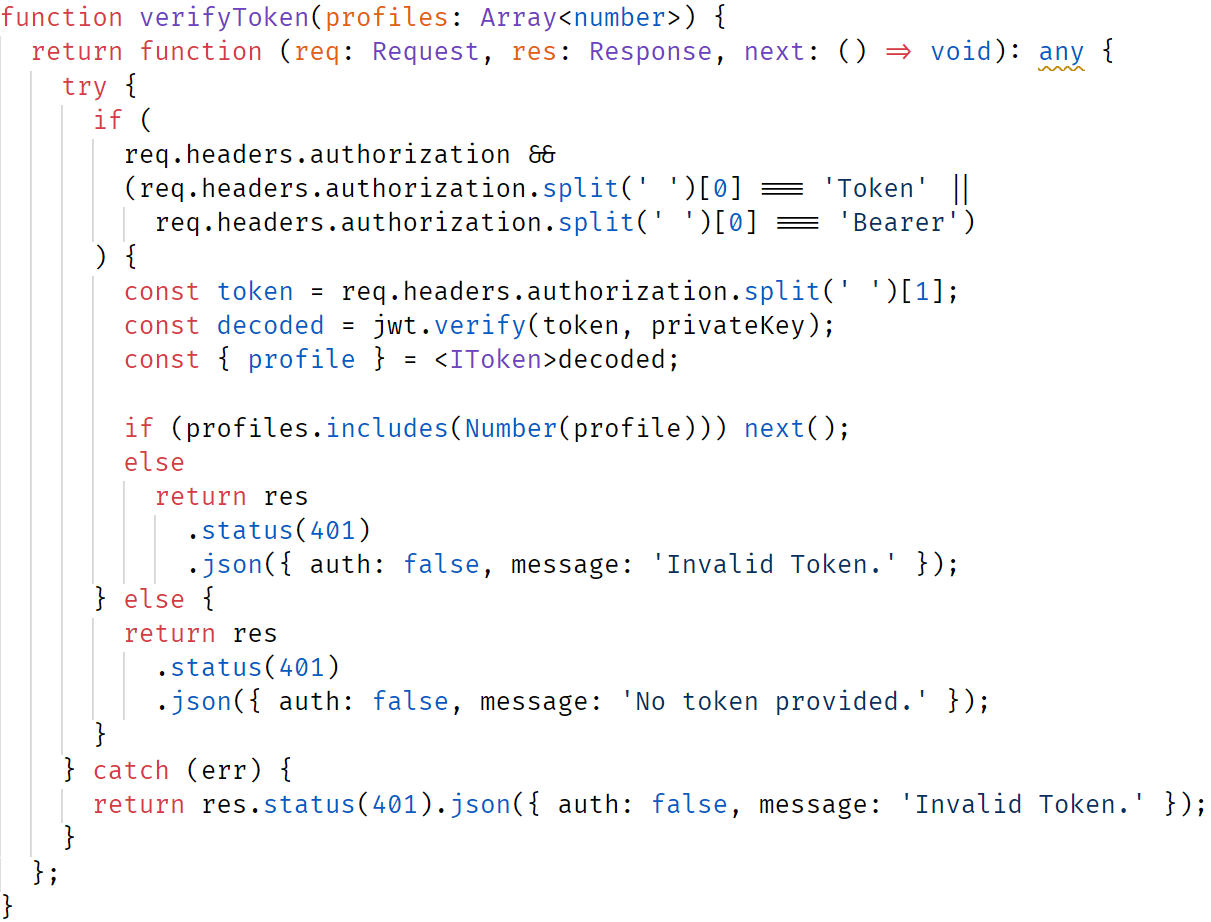
\includegraphics[width=\textwidth]{dados/figuras/Proposta/Códigos/code_validate_token.png}
    \caption{Geração de Tokens usando JWT}
    \label{fig:codigoValidadorDeToken}
\end{figure}


\subsection{\textit{Front-end}}

\cite{roveda2018frontend} descreve \textit{\textit{Front-end}} como toda parte da programação relativa à interface de uma aplicação e com o qual o usuário é capaz de interagir com o sistema. O \textit{\textit{Front-end}} KeeMe, como foi construído utilizando como base a biblioteca React que como descrito por sua documentação em \cite{react} se trata de uma biblioteca JavaScript para construção de interfaces. Em conjunto ao React, optou-se por utilizar também a biblioteca ChakraUI, que é "uma biblioteca de componentes simples, modular e acessível que fornece os blocos de construção de que você precisa para construir seus aplicativos React" \cite{chakraui}. A etapa de criação do \textit{\textit{Front-end}} buscou criar uma interface que fosse simples e de fácil utilização de forma que os usuários pudessem utilizá-la sem a necessidade de intervenção ou de tutoriais, além isso utilizou-se uma palheta de cores com a predominância do verde, que na psicologia das cores descrita por \cite{clemente2020cores} está relacionada à sensação de relaxamento e harmonia, dessa forma a interface busca passar ao usuário a sensação de relaxamento durante a utilização do sistema.

\begin{figure}[H]
    \centering
    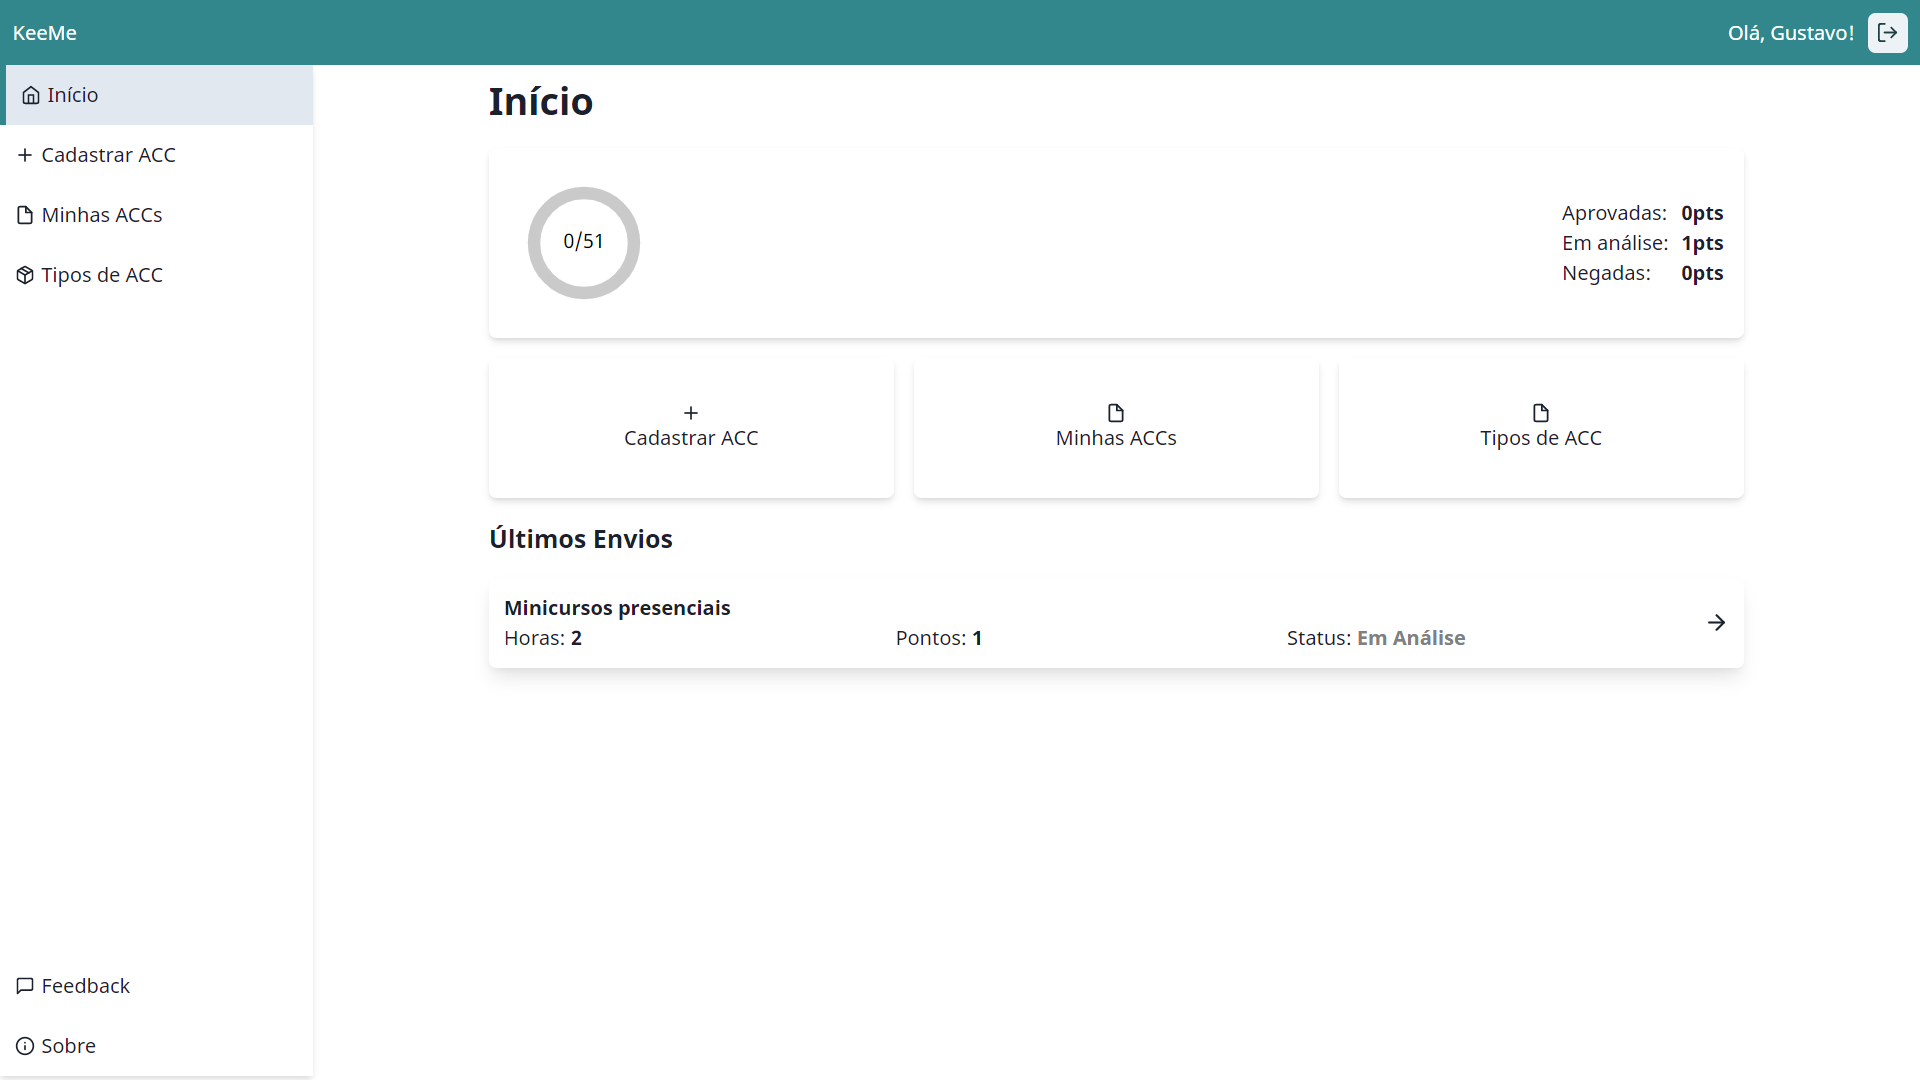
\includegraphics[width=\textwidth]{dados/figuras/Proposta/Screens/student_dashboard.png}
    \caption{Tela de Início do Discente}
    \label{fig:screenDashboardDiscente}
\end{figure}

A Figura \ref{fig:screenDashboardDiscente} mostra a tela de início de um usuário do tipo Discente, essa tela possui um resumo de todos os dados do discente. Trazendo um gráfico que mostra o avanço do discente em relação à conclusão da pontuação de ACC assim como a quantidade de pontos Aprovados, Em análise e Negados. Também são mostradas as principais funcionalidades do sistema, sendo estas Cadastrar ACC, Minhas ACCs e Tipos de ACC, além de uma seção com os últimos envios realizados pelo discente.

\begin{figure}[H]
    \centering
    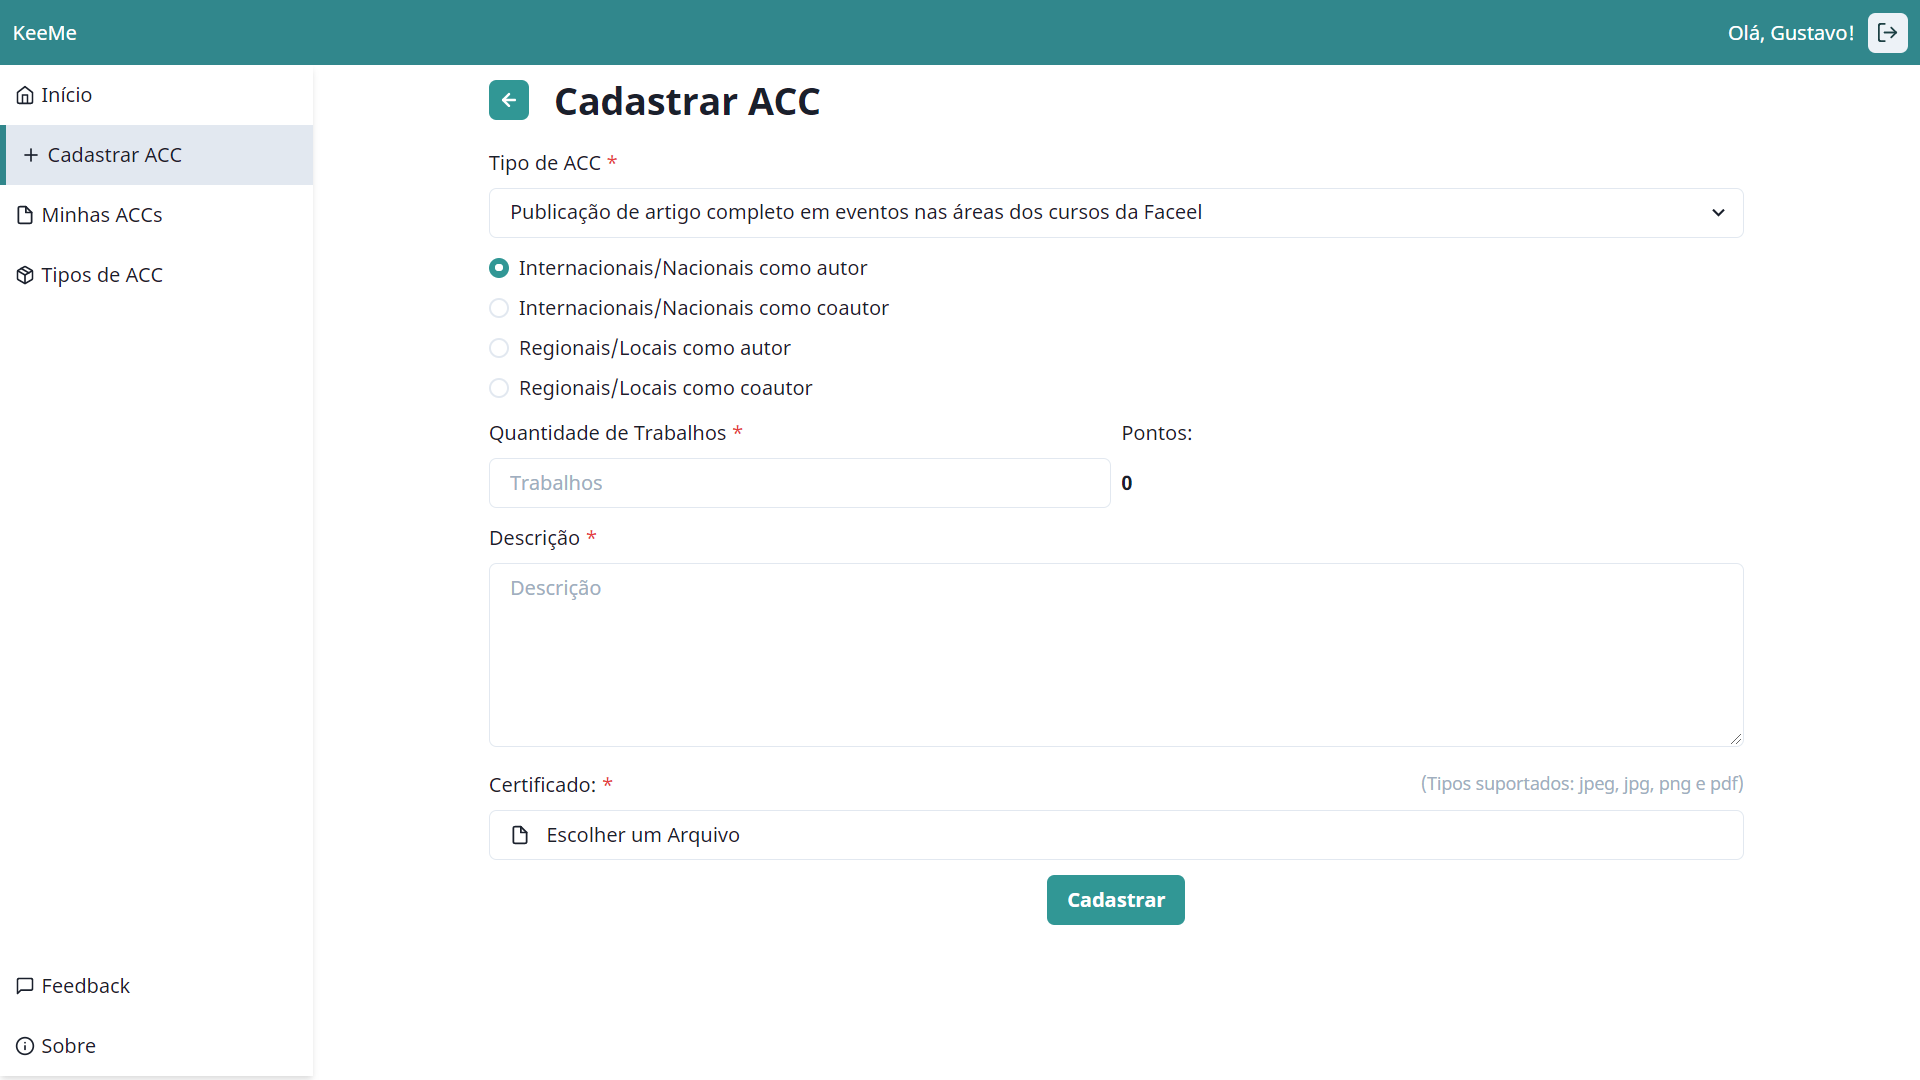
\includegraphics[width=\textwidth]{dados/figuras/Proposta/Screens/student_acc_request.png}
    \caption{Tela de Cadastro de ACC}
    \label{fig:screenCadastrarACC}
\end{figure}

Na Figura \ref{fig:screenCadastrarACC} é mostrada a tela de cadastro de uma ACC realizada pelo discente. O discente deve escolher um Tipo de ACC, e caso haja variações (Relacionado aos cursos da Faceel ou Não Relacionado aos cursos da Faceel, Congresso Regional ou Nacional, entre outros), deve escolher entre as mesmas. Além disso, o discente deve preencher a quantidade de unidades (como horas, semestres, dentre outros) realizadas, escrever uma descrição sobre a ACC, ou seja, o que ele realizou na mesma e por último anexar um certificado referente à ACC.

\begin{figure}[H]
    \centering
    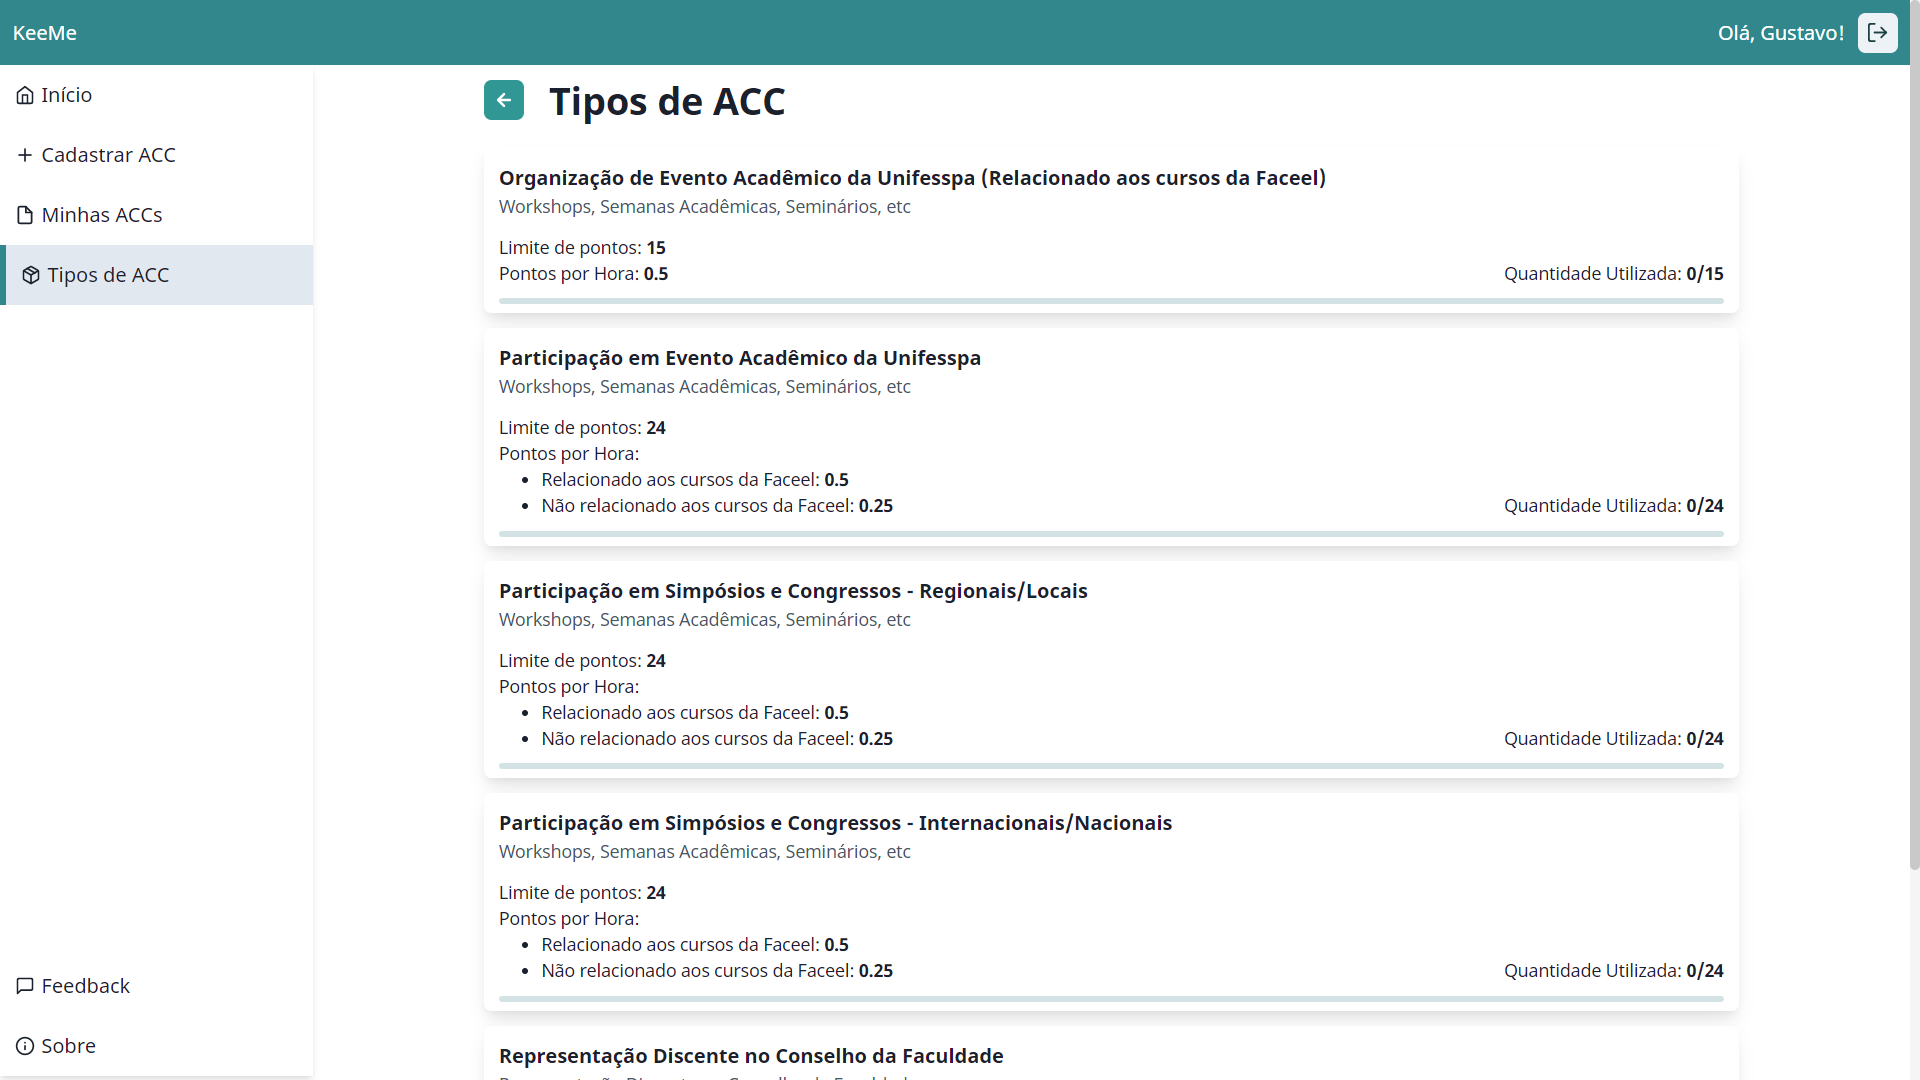
\includegraphics[width=\textwidth]{dados/figuras/Proposta/Screens/student_acc_types.png}
    \caption{Tela de Tipos de ACC}
    \label{fig:screenTiposDeACC}
\end{figure}

O discente poderá acessar os dados dos Tipos de ACC presentes no regulamento, assim como suas descrições, pontos por unidade e limites. Além disso, o discente poderá acompanhar visualmente quantos pontos o mesmo já conseguiu em determinado tipo de ACC, conforme mostrado na Figura \ref{fig:screenTiposDeACC}.

\begin{figure}[H]
    \centering
    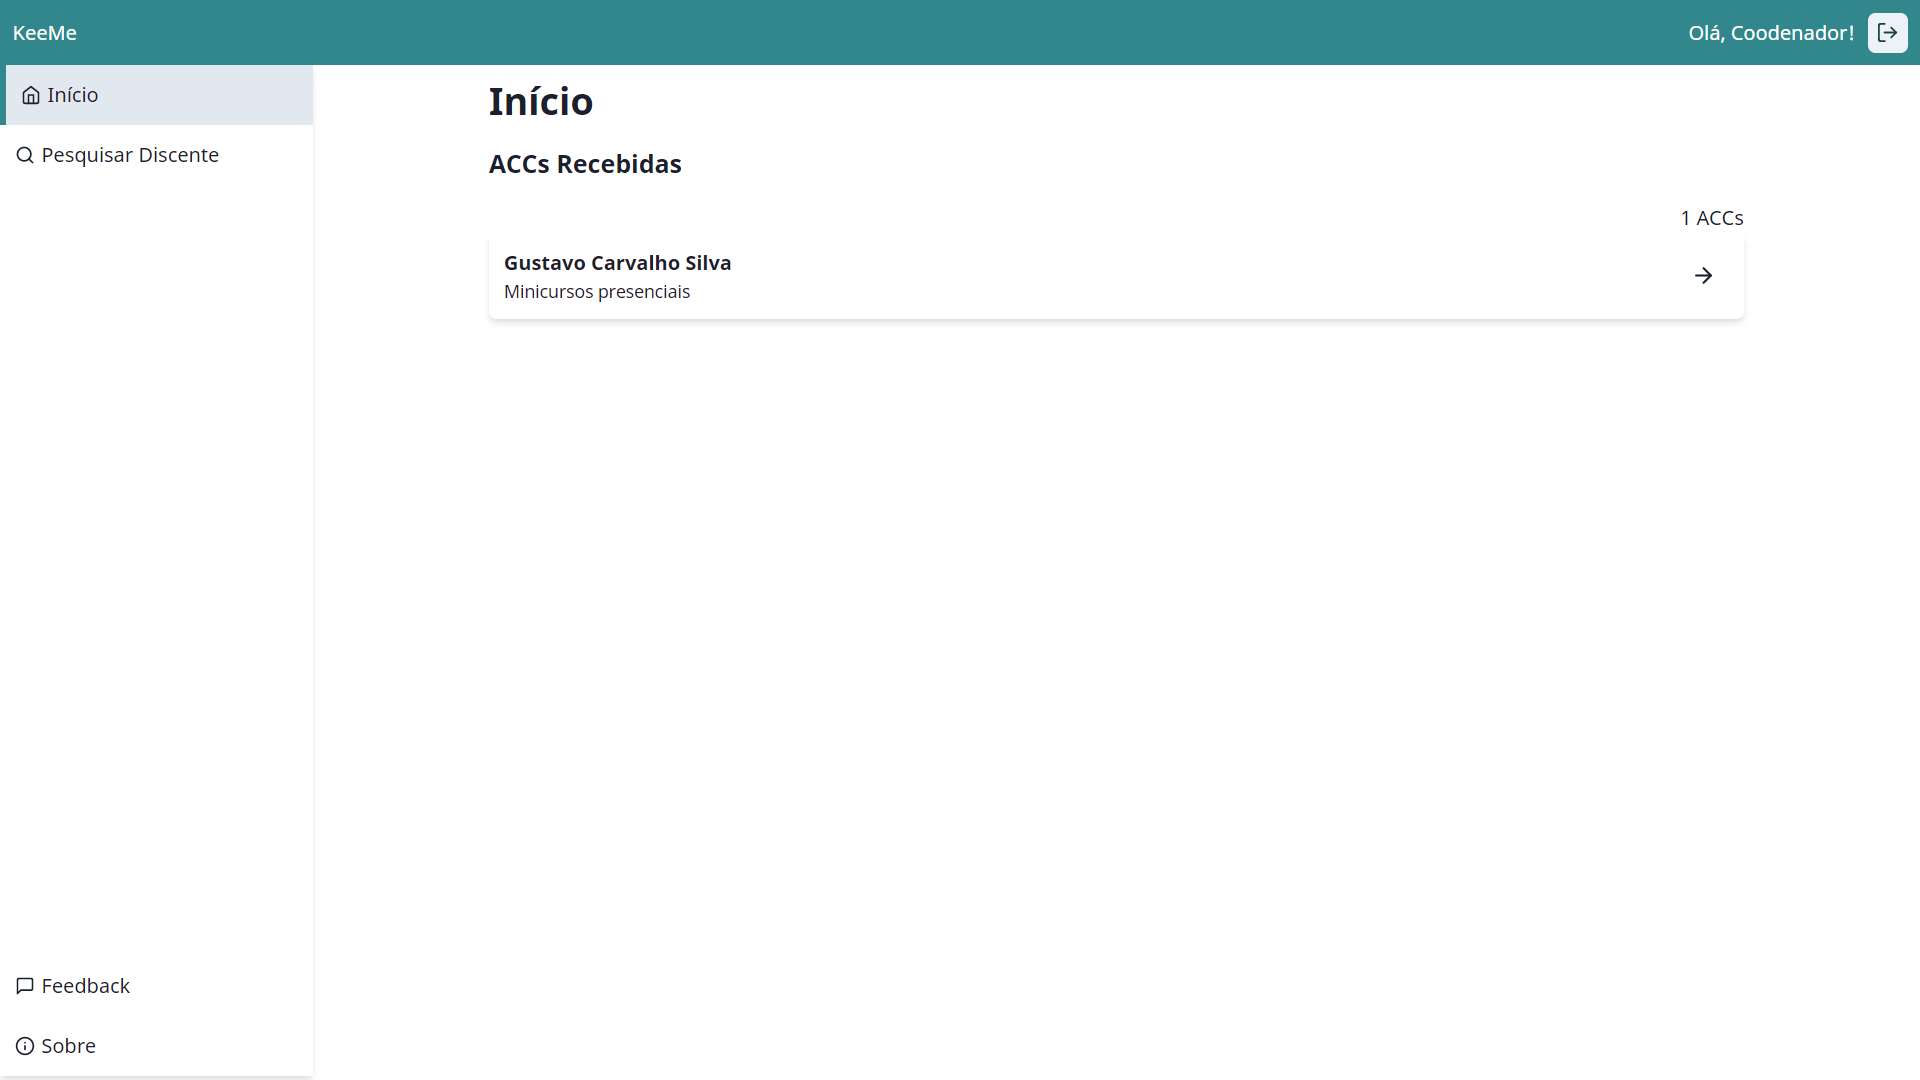
\includegraphics[width=0.9\textwidth]{dados/figuras/Proposta/Screens/coordinator_received_accs.png}
    \caption{Tela de Início do Coordenador}
    \label{fig:screenACCsRecebidas}
\end{figure}

A Figura \ref{fig:screenACCsRecebidas} mostra a tela de início de um usuário do tipo coordenador, conforme mostrado na imagem, o coordenador poderá ver as ACCs enviadas pelos discentes do curso ao qual ele está vinculado, além de uma contagem do número de ACCs que ainda precisam ser avaliadas.

\begin{figure}[H]
    \centering
    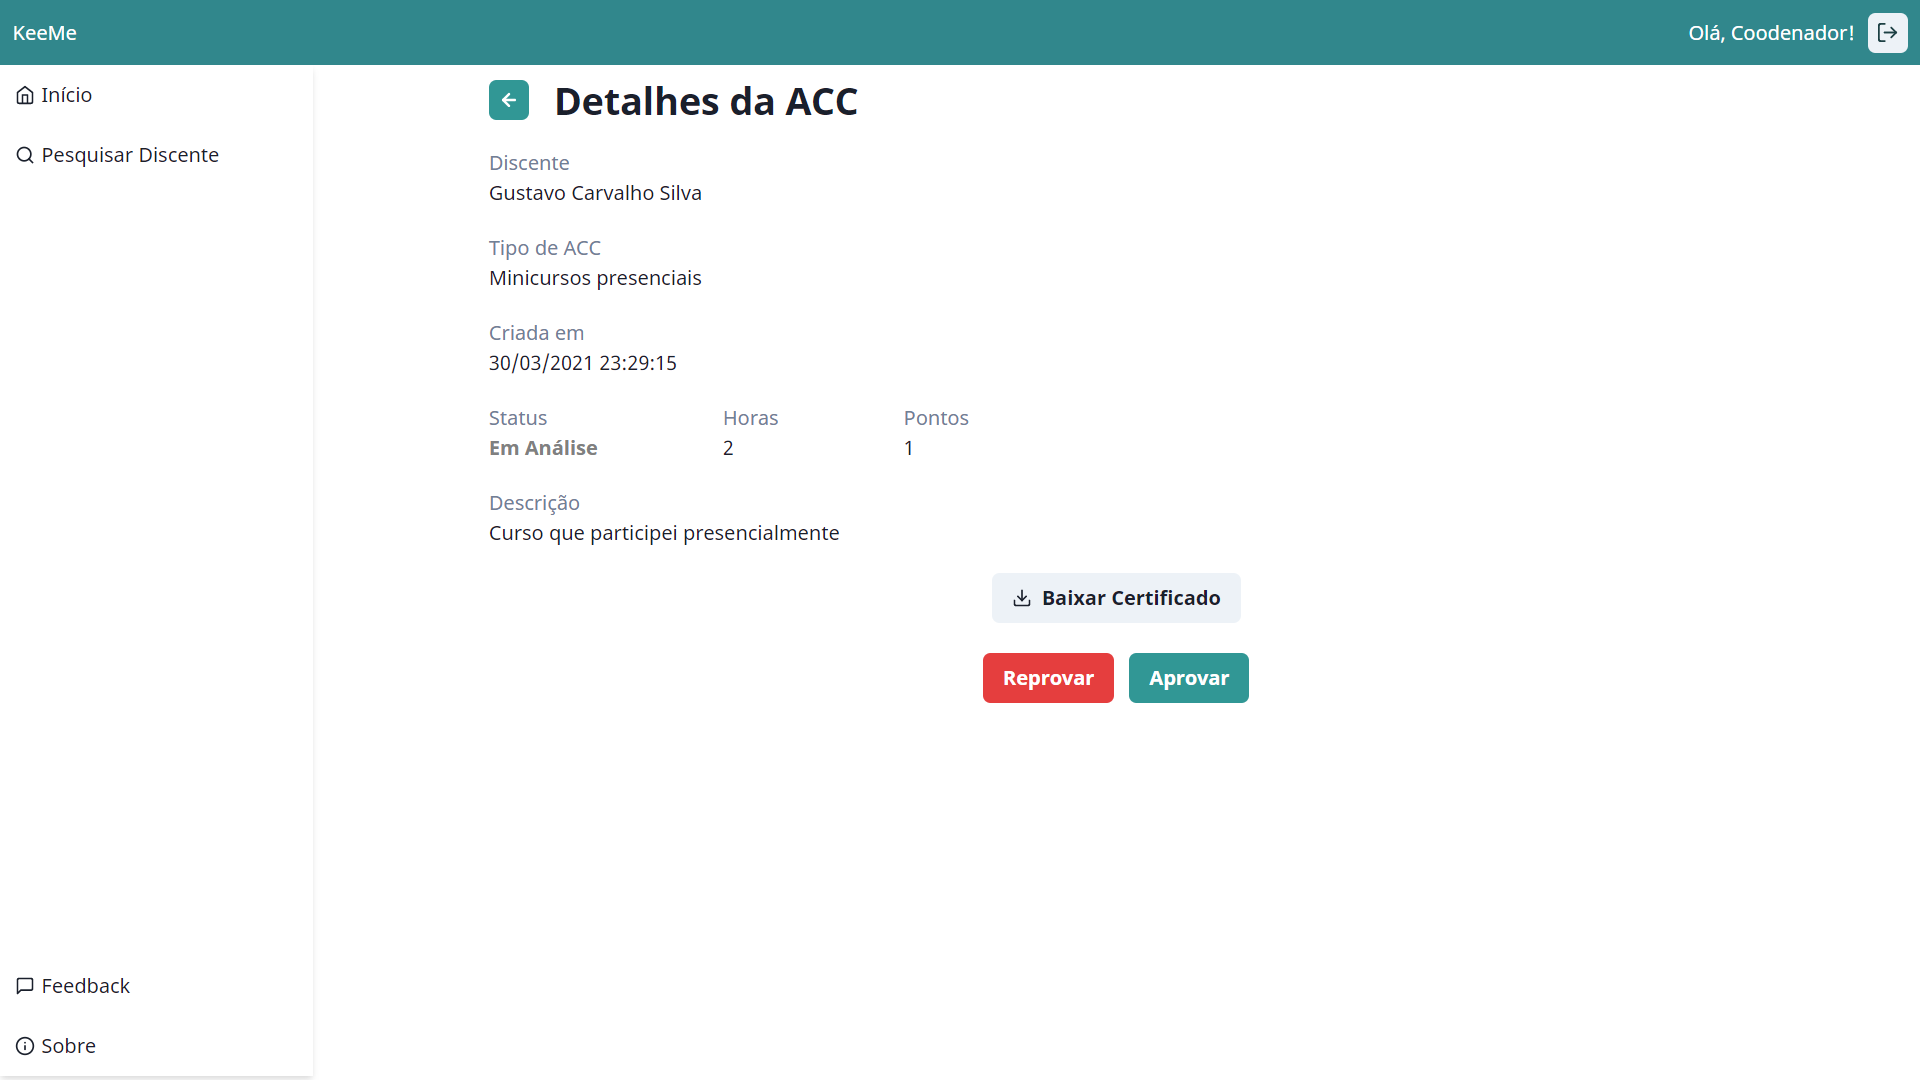
\includegraphics[width=0.9\textwidth]{dados/figuras/Proposta/Screens/evaluate_acc.png}
    \caption{Tela de Avaliação das ACCs}
    \label{fig:screenAvaliarACC}
\end{figure}

Na Figura \ref{fig:screenAvaliarACC} é possível ver a tela de avaliação de uma ACC. Como pode ser visto na imagem, além dos dados da ACC, o Coordenador poderá também baixar o certificado anexado. Após chegar a uma decisão, o Coordenador poderá aprovar a ACC ou reprová-la. No caso de uma reprovação, o coordenador deverá escrever o motivo da sua decisão.

\begin{figure}[H]
    \centering
    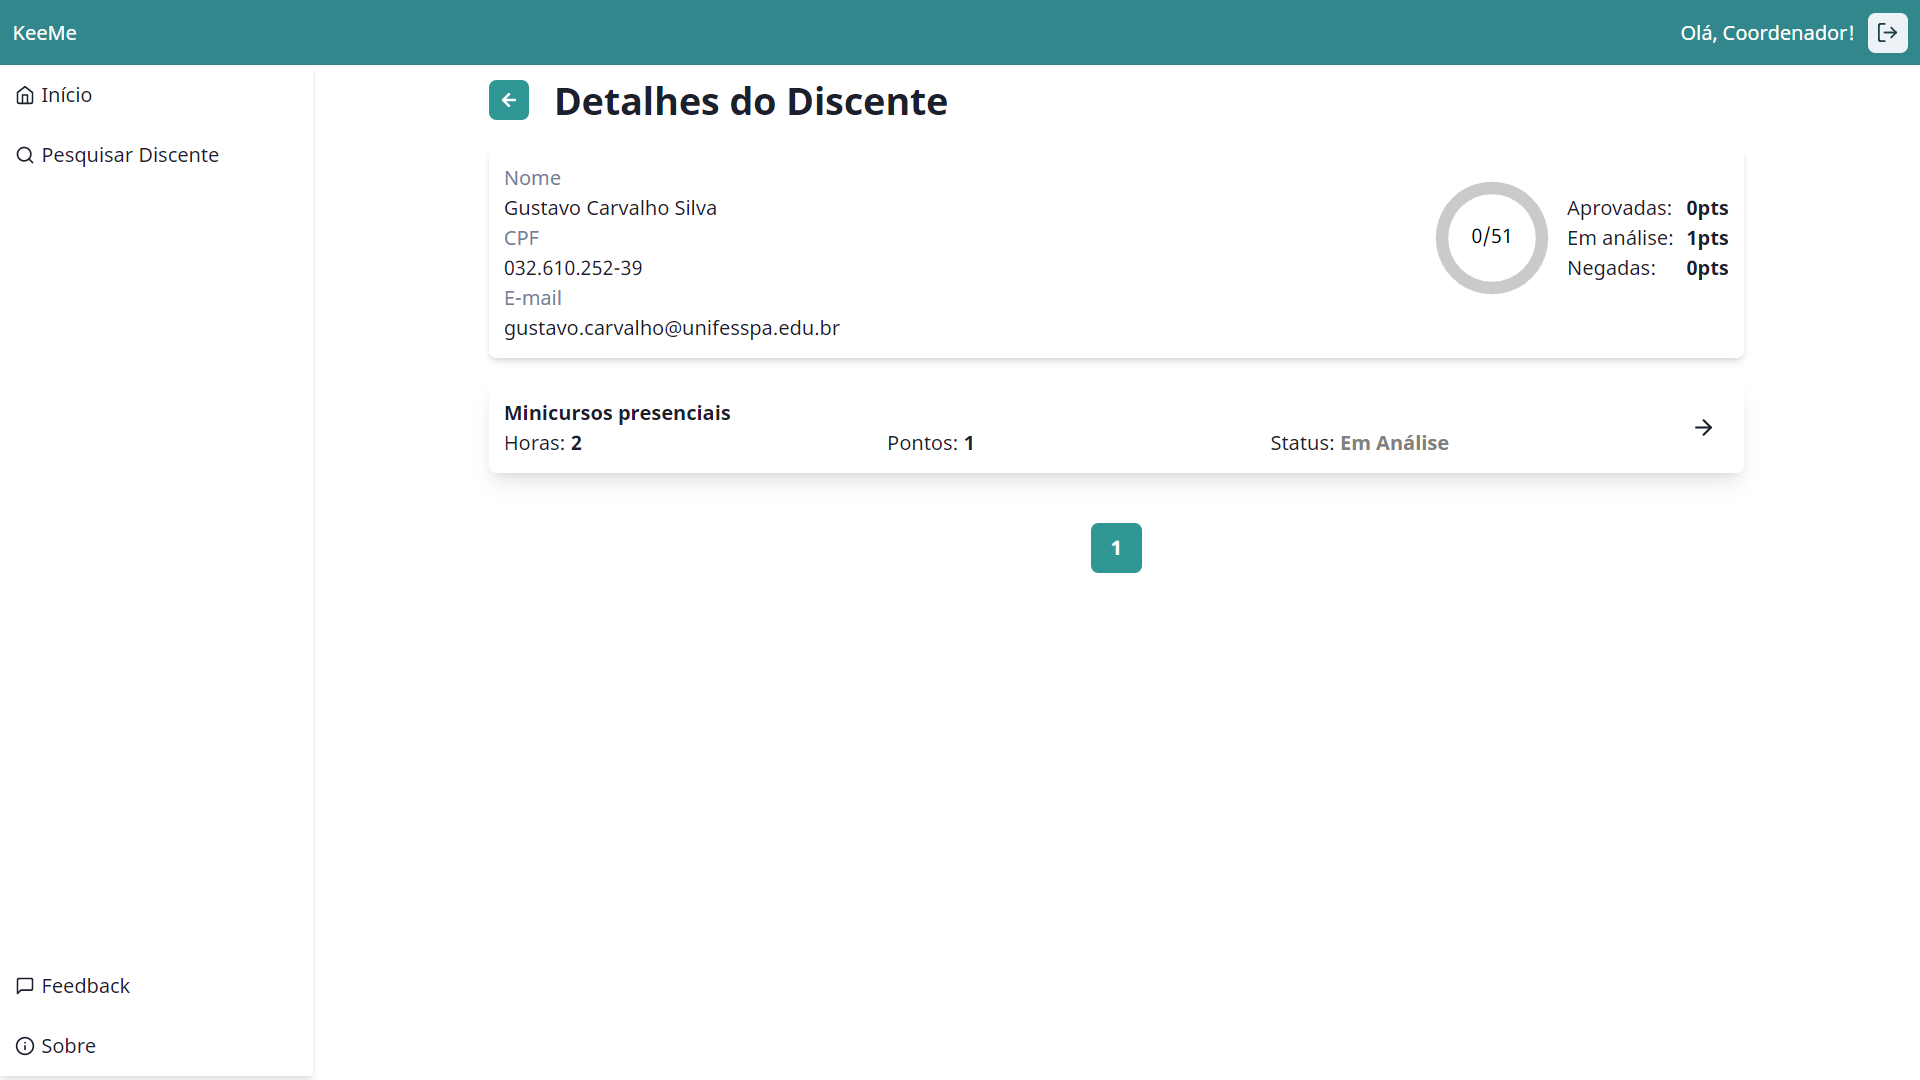
\includegraphics[width=\textwidth]{dados/figuras/Proposta/Screens/coordinator_student_details.png}
    \caption{Tela de Detalhes do Discente}
    \label{fig:screenDetalhesDoDiscente}
\end{figure}

O coordenador poderá acompanhar o avanço de um discente através da tela mostrada na Figura \ref{fig:screenDetalhesDoDiscente}. Essa tela exibe todas as informações pertinentes de um discente, além das informações de pontuação do mesmo. Sedo assim, é mostrado um gráfico que ilustra o avanço do discente na pontuação, e a quantidade de pontos que o mesmo possui para diferentes estados tais como, "Aprovados", "Reprovados" e "Em análise".

\begin{figure}[H]
    \centering
    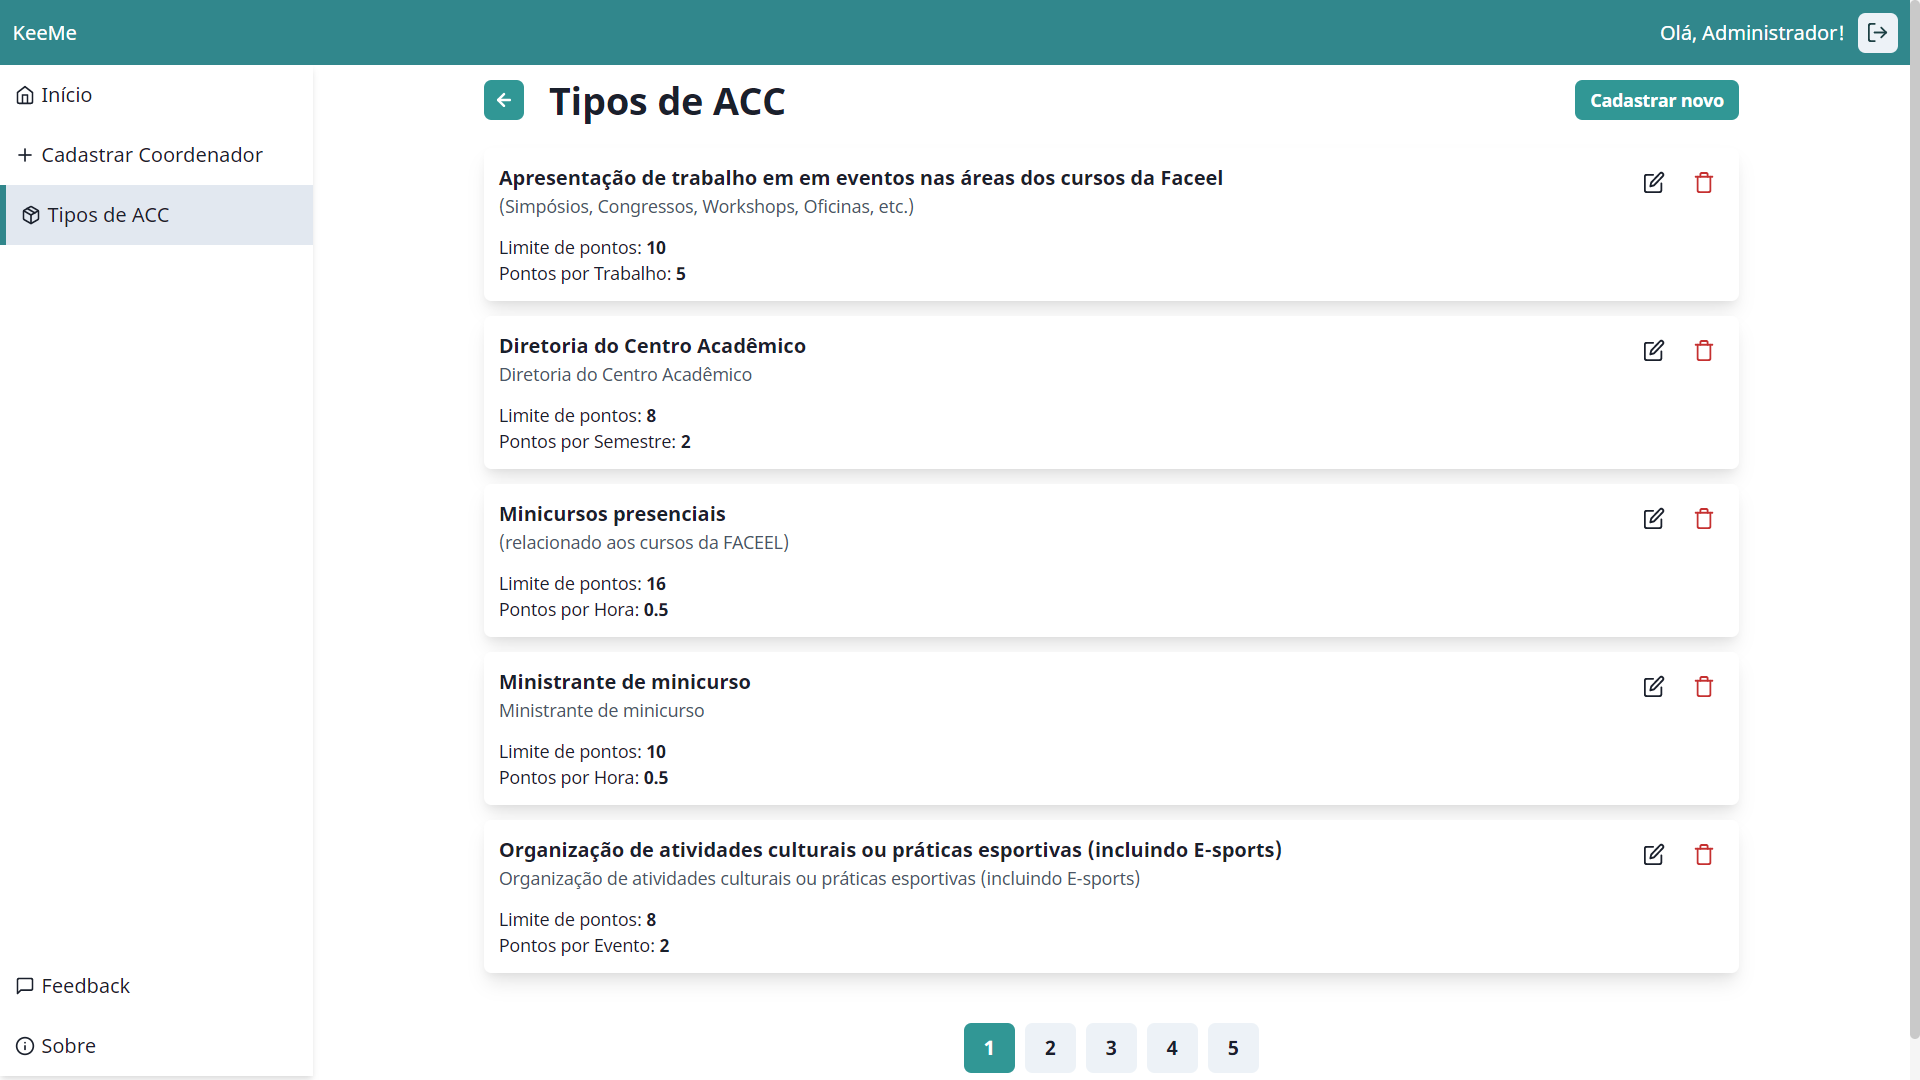
\includegraphics[width=\textwidth]{dados/figuras/Proposta/Screens/admin_acc_types.png}
    \caption{Tela de Listagem dos Tipos de ACC}
    \label{fig:screenListagemTiposDeACC}
\end{figure}

A Figura \ref{fig:screenListagemTiposDeACC} mostra a tela de listagem dos Tipos de ACC, esta tela se encontra dentro do módulo do Administrador e está baseada no caso de uso expandido da Tabela \ref{casoExpandido:gerenciarTiposDeACC}. Através dessa tela o Administrador tem acesso aos Tipos de ACC presentes dentro do sistema, além de poder realizar as operações de Cadastro, Consulta, Edição e Exclusão.

\begin{figure}[H]
    \centering
    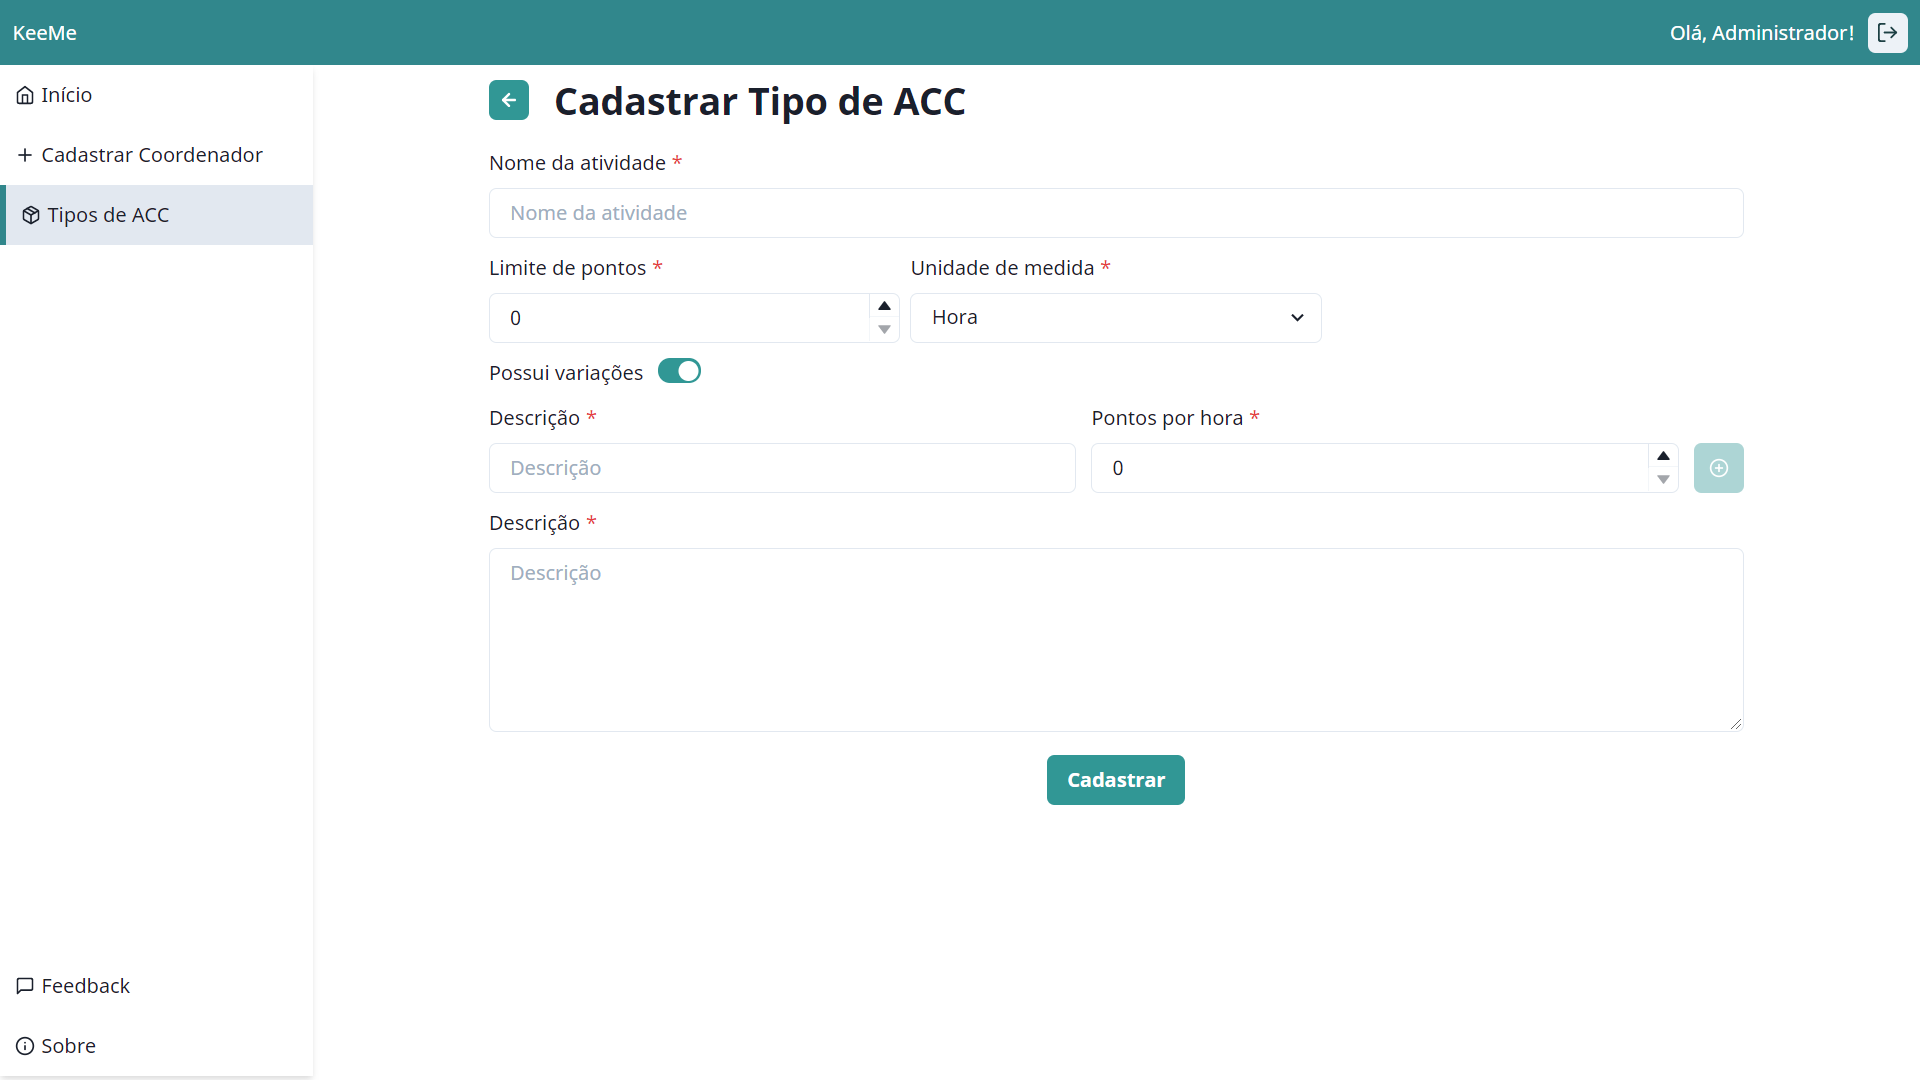
\includegraphics[width=\textwidth]{dados/figuras/Proposta/Screens/admin_create_acc_type.png}
    \caption{Tela de Cadastro de Tipo de ACC}
    \label{fig:screenCadastroTipoDeACC}
\end{figure}

Na Figura \ref{fig:screenCadastroTipoDeACC} é possível ver a tela de Cadastro de um novo Tipo de ACC, ação realizada por um usuário do tipo Administrador. O Administrador deve preencher os campos: Nome da atividade; Limite de pontos, que descreve o máximo de pontos que um usuário pode obter no Tipo de ACC; Unidade de Medida, que é a forma em que o Tipo de ACC será pontuado, se por Horas, Semestres, Certificados, entre outros; Variações, que são as variantes que este Tipo de ACC pode possuir, como Congresso Regional ou Nacional, dentro dos cursos da FACEEL ou não, entre outros; e a descrição do Tipo de ACC; Como pode ser observado na Figura \ref{fig:screenCadastroTipoDeACC} há uma opção chamada "Possui variações", caso essa opção esteja desmarcada o sistema não exibirá os campos para se adicionar as variantes, ficando apenas o campo de número de Pontos por unidade de medida, dessa forma, o Tipo de ACC será salvo sem variações.
